\documentclass[11pt, a4paper]{report}

\usepackage[english, french]{babel}
\usepackage[T1]{fontenc}
\usepackage[latin1]{inputenc}
%\usepackage{ucs}
\usepackage{lmodern}
\usepackage{url} % Pour avoir de belles url
\usepackage{geometry}
%\usepackage{slashbox} %backslash dans tableau
\usepackage[table, usenames, dvipsnames]{xcolor} %couleurs
\usepackage{colortbl,hhline}
\usepackage{color}
\usepackage{listings} % Pour mettre du code source
%\usepackage{lscape} %Pour pouvoir passer en paysage
%\usepackage {multicol} %Pour pouvoir faire plusieurs colonnes
%\usepackage{eurosym} %symbole euro
\usepackage{graphicx}
\usepackage{makeidx} %Pour crer un index
%\usepackage{setspace} %Pour l'interligne de 1.5
%\usepackage{shorttoc} %Pour crer un sommaire
%\usepackage{caption}
%\usepackage[font=scriptsize, format=hang]{subcaption}
%\usepackage[babel=true]{csquotes}
\usepackage{extensions/picins} %image avec texte a ct
\usepackage[toc,page]{extensions/appendix}
\usepackage{extensions/subfig}
\usepackage{extensions/capt-of}
\usepackage{fancyhdr} % Pour les entetes de page
\usepackage[
	pdftex,					% Paramtrage de la navigation
	bookmarks = true,						% Signets
	bookmarksnumbered = true,				% Signets numrots
	pdfpagemode = UseOutlines,						% None, UseThumbs, UseOutlines, Fullscreen
	pdfstartview = Fit,					% FitH, FitV, FitR, FitB, FitBH, FitBV, Fit
	pdfpagelayout = SinglePage,				% SinglePage, OneColumn, TwoColumnLeft, TwoColumnRight
	colorlinks = false,					% Liens en couleur
	urlcolor = black,						% Couleur des liens externes
	pdfborder = {0 0 0}					% Style de bordure : ici, rien
]{hyperref}

\lstset{
	numbers=left,
	numberstyle=\footnotesize,
	stepnumber=2,
	numbersep=5pt,
	frame=shadowbox,
	backgroundcolor=\color{grisclair},
	rulesepcolor=\color{gris},
	keywordstyle=\color{darkblue},
	captionpos=b,
	showstringspaces=false,
	numberfirstline=true
}

\lstdefinelanguage{LQL}{
	showspaces=false,
	identifierstyle=\color{black},
	captionpos=b
}

\lstdefinelanguage{JSON}{
	showspaces=false,
	morestring=[b]", %pour les guillemets en bleu
	morecomment=[s]{"?}{?"}, %contenu des guillemets en bleu
	stringstyle=\color{darkblue},
	captionpos=b
}

\lstdefinelanguage{XML}{
	showspaces=false,
	morestring=[b]",
	morestring=[s]{>}{<},
	morecomment=[s]{<?}{?>},
	stringstyle=\color{black},
	identifierstyle=\color{darkblue},
	keywordstyle=\color{cyan},
	morekeywords={id,value,onClick},
	captionpos=b
}

\lstdefinelanguage{plaintext}{
	morekeywords={@}, 
	keywordstyle=\color{darkblue}, 
	captionpos=b
}

\renewcommand{\labelitemi}{---}
\renewcommand{\labelitemii}{$\star$}

\newcommand\Yuukou{\textit{Yuukou}}
\newcommand\YuukouII{\textit{Yuukou II}}
\newcommand\cad{c'est-\`a-dire}

\renewcommand{\appendixtocname}{Annexes}
\renewcommand{\appendixpagename}{Annexes}

\hypersetup{
	unicode=false,          % non-Latin characters in Acrobat's bookmarks
	pdftoolbar=true,        % show Acrobat's toolbar?
	pdfmenubar=true,        % show Acrobat's menu?
	pdffitwindow=true,     % window fit to page when opened
	pdftitle={Rapport de stage},    % title
	pdfauthor={Meilhac Benoît},     % author
	pdfsubject={Yuukou II},   % subject of the document
	pdfcreator={Meilhac Benoit},   % creator of the document
	pdfproducer={Texlive (pdflatex)}, % producer of the document
	pdfnewwindow=true,      % links in new window
}


\graphicspath{{images/}}
\newcommand{\sommaire}{\shorttoc{Sommaire}{0}}
\makeindex
\definecolor{grisclair}{gray}{0.75}
\definecolor{gris}{gray}{0.5}
\definecolor{orange}{rgb}{1,0.5,0}
\definecolor{vert}{rgb}{0,0.75,0}
\definecolor{darkblue}{rgb}{0.0,0.0,0.6}
\definecolor{cyan}{rgb}{0.0,0.6,0.6}

% Pour les marges de la page
%\geometry{a4paper, top=2.5cm, bottom=3.5cm, left=1.5cm, right=1.5cm, marginparwidth=1.2cm}
\geometry{a4paper}

\parskip=5pt %% distance entre les (paragraphe)
\sloppy %% respecter toujours la marge de droite 

% Pour les pénalités :
\interfootnotelinepenalty=150 %note de bas de page
\widowpenalty=150 %% veuves et orphelines
\clubpenalty=150 

%Pour la longueur de l'indentation des paragraphes
\setlength{\parindent}{15mm}

%%%% debut macro pour enlever le nom chapitre %%%%
\makeatletter
	\def\@makechapterhead#1{%
		\vspace*{50\p@}%
		{\parindent \z@ \raggedright \normalfont
			\interlinepenalty\@M
			\ifnum \c@secnumdepth >\m@ne
			\Huge\bfseries \thechapter\quad
			\fi
			\Huge \bfseries #1\par\nobreak
			\vskip 40\p@
		}}

	\def\@makeschapterhead#1{%
		\vspace*{50\p@}%
		{\parindent \z@ \raggedright
			\normalfont
			\interlinepenalty\@M
			\Huge \bfseries  #1\par\nobreak
			\vskip 40\p@
		}
	}
\makeatother
%%%% fin macro %%%%

\begin{document}
\pagestyle{empty}
\begin{titlepage}
    \centering

    \vspace{5mm}

	\normalsize{
		\textbf{
			D\'epartement informatique\\
			Universit\'e de France-Comt\'e\\
			Stage du 13 f\'evrier au 4 juin\\
			Ann\'ee 2011-2012
		}
	}

    \vspace{5mm}
	
    \Huge{
        \textbf{
            Projet Yuukou II
        }
    }

    \vspace{5mm}

    \normalsize{
        Beno\^it MEILHAC
    }

    \vspace{5mm}
	
    \begin{center} 
        
\includegraphics[scale=0.3]{westminsterLogo.jpg}
	\end{center}
	
    \vspace{14mm}

    \Huge{
        \textbf{
            Rapport de stage
        }
	}

	\vspace{20mm}

    \normalsize{
        \textbf{
			School of Electronics and Computer Science\\
            University of Westminster\\
        	115 New Cavendish Street\\
			London W1W 6UW\\
        }
    }

	\vspace{5mm}

	\normalsize{	
	    Tuteur de stage : M. DELAITRE\\
		Responsable de stage : M. HUFFLEN
	}

\end{titlepage}

\clearpage



\pagenumbering{Roman} 
\setcounter{page}{1} 

\chapter*{Remerciements}
\addcontentsline{toc}{chapter}{Remerciements}

Je tiens avant tout \`a remercier mon tuteur de stage M. Thierry DELAITRE pour son accueil \`a l'Universit\'e, pour m'avoir propos\'e un projet aussi int\'eressant, pour avoir mis \`a ma disposition tout ce dont j'avais besoin pour travailler correctement et aussi pour tout le temps qu'il m'a consacr\'e.

Je remercie \'egalement mon responsable de stage M. Jean-Michel HUFFLEN pour m'avoir offert l'opportunit\'e d'effectuer mon stage de fin d'\'etudes \`a Londres mais aussi pour ses conseils et l'aide apport\'ee pendant la r\'edaction de ce rapport.

J'adresse aussi tous mes remerciements \`a toute l'\'equipe du CPC, avec qui j'ai partag\'e un bureau, pour m'avoir accueilli, pour leur aide et leur bonne humeur malgr\'e la barri\`ere de la langue en d\'ebut de stage.

Merci encore \`a mes camarades francophones Damien HOSTACHE et Yacine MAGHEZZI venus me rejoindre en cours de stage pour les bons moments pass\'es ensemble.

J'exprime \'egalement toute ma gratitude \`a C\'elia NASROUNE et J\'er\'emie BOURSEAU pour le travail de relecture qu'ils ont effectu\'e et l'aide apport\'ee.

\clearpage


\tableofcontents
\clearpage

\pagestyle{fancy}
\renewcommand{\chaptermark}[1]{\markboth{#1}{}} 
\renewcommand{\sectionmark}[1]{\markright{#1}} 
\pagenumbering{arabic} 
\setcounter{page}{1} 

\chapter*{Introduction}
\addcontentsline{toc}{chapter}{Introduction}

Le cursus professionnel de deuxi\`eme ann\'ee du Master informatique \`a l'Universit\'e de Franche-Comt\'e de Besan\c{c}on inclut la r\'ealisation d'un stage en entreprise d'une dur\'ee minimum de quatre mois. 
L'Universit\'e donne, de plus, l'opportunit\'e d'effectuer ce stage \`a l'\'etranger.

L'anglais est la langue pr\'edominante dans le domaine de l'informatique mais c'est aussi un pr\'e-requis indispensable dans certaines recherches d'emploi.
C'est pour cela que j'ai saisi la chance qu'offrait l'Universit\'e pour r\'ealiser mon stage au Royaume-Uni. 
C'est avec l'aide de M. Jean-Michel HUFFLEN, Ma\^itre de Conf\'erences \`a l'Universit\'e de Franche-Comt\'e, que j'ai pu int\'egrer pendant quatre mois l'Universit\'e de Westminster \`a Londres o\`u j'ai \'et\'e accueilli par M. Thierry DELAITRE, directeur des infrastructures \`a l'Universit\'e, afin de travailler sur le projet \YuukouII.

Ce projet est n\'e d'une collaboration de deux \'equipes de l'Universit\'e : l'\textit{Infrastructure Team} de la \textit{School of Electronics and Computer Science} et les services centraux informatiques \textit{Information Systems and Library Services}. 
De ce fait, j'ai int\'egr\'e ces deux \'equipes tout en travaillant dans le \textit{Centre for Parallel Computing}.

\Yuukou, venant du japonais et signifiant validit\'e, disponibilit\'e, efficacit\'e, est un projet mis en place dans le but de montrer l'utilisation des salles informatiques et d'en garder un historique.
Ainsi, il permet de conna\^itre la disponibilit\'e des salles de l'Universit\'e et offre la possibilit\'e de voir les ordinateurs disponibles, occup\'es ou encore \'eteints.

Cependant les principaux d\'eveloppeurs de cette application ne faisant plus partie de l'Universit\'e, le projet n'est plus maintenu.
De plus, son principal int\'er\^et serait de faire savoir \`a un \'etudiant les salles qui sont disponibles ainsi que les ordinateurs libres.
Ce qu'il ne fait que tr\`es partiellement actuellement.
En outre, l'Universit\'e change le fonctionnement de son infrastructure, ce qui aura, entre autres cons\'equences de rendre l'application obsol\`ete.

C'est dans ce contexte que s'inscrit le projet \YuukouII. 
Mon stage consiste donc \`a la mise en place d'un service Web permettant le suivi des diff\'erents ordinateurs de l'Universit\'e et pouvant retourner ces donn\'ees pour un affichage sur un \textit{smartphone}, ou encore un \'ecran plasma se trouvant \`a l'entr\'ee de chaque b\^atiment par exemple.

Le pr\'esent rapport concerne le travail r\'ealis\'e au sein de l'Universit\'e de Westminster.
Une premi\`ere partie pr\'esentera l'Universit\'e et les services que j'ai int\'egr\'es ainsi que ceux que j'ai c\^otoy\'es tout au long du stage.
Une seconde partie traitera du projet \Yuukou{}, avec une pr\'esentation de ses fonctionnalit\'es et de ce \`a quoi il donne acc\`es  ainsi que des raisons qui ont conduit au projet \YuukouII.
Cette partie abordera aussi la d\'ecouverte du sujet de stage.
Une troisi\`eme partie permettra de d\'ecouvrir le sujet avec plus de d\'etails afin de comprendre les choix qui ont \'et\'e r\'ealis\'es dans les autres parties du rapport.
La quatri\`eme partie mettra en avant la notion de service Web, le point central du projet.
Ensuite, une cinqui\`eme partie pr\'esentera les diff\'erentes recherches qui ont \'et\'e faites, le travail accompli et les probl\`emes rencontr\'es.
Enfin, une derni\`ere partie donnera un bilan des diff\'erents points retenus lors de ce stage avant de clore ce rapport.

\vspace{1.5cm}

\begin{center}
\textit{\underline{NOTE} : Les termes marqu\'es d'une ast\'erisque($^*$) sont d\'efinis dans le glossaire.}

\end{center}

\clearpage


\chapter{Lieu de stage}

\section{University of Westminster}

\subsection{Pr\'esentation}

\parpic{
	\begin{minipage}{0.27\textwidth}
		
\includegraphics[scale=1.0]{westminsterBlason.jpg}
		\caption{Blason de l'universit\'e}
	\end{minipage}}
L'Universit\'e de Westminster est une universit\'e publique de recherche situ\'ee \`a Londres. 
\`A sa fondation, en 1838, elle portait le nom de \textit{Royal Polytechnic Institution} et \'etait la premi\`ere \'ecole polytechnique ouverte en Angleterre.
Son but \'etait de fournir une institution o\`u le public peut, \`a moindre co\^ut, acqu\'erir une connaissance pratique des divers arts et branches de la science en rapport avec les fabricants industriels, les op\'erations mini\`eres et l'\'economie rurale.
Sa fondation est une r\'eaction \`a la popularit\'e grandissante de l'enseignement de type polytechnique en europe continentale. 
Notamment avec l'Allemagne et la \textit{Fachhochschule}, la France et l'\textit{\'Ecole Polytechnique} ou encore les \'Etats-Unis et la \textit{Rensselaer Polytechnic Institute}.

En 1970, la \textit{Royal Polytechnic Institution} devient \textit{Polytechnic of Central London} apr\`es avoir fusionn\'e avec \textit{Holborn College of Law, Languages and Commerce}.
C'est en 1992 que le statut d'universit\'e fut attribu\'e \`a Westminster qui devint \textit{University of Westminster}.

\subsection{Les diff\'erents campus et \'ecoles}
\label{section:campus}

L'universit\'e compte quatre principaux campus, trois dans le centre de Londres : Regent, Cavendish, Marylebone et le quatri\`eme \`a Harrow, \`a l'ouest de Londres.

\begin{itemize}
	\item \textbf{Regent} : situ\'e au 309 Regent Street, c'est le campus le plus ancien de l'universit\'e, il contient une \'ecole : 
		\textit{School of Social Sciences, Humanities and Languages};

	\item \textbf{Cavendish} : situ\'e au 101-115 New Cavendish Street, dans le quartier de Fitzrovia proche de West End de Londres (entre Marylebone, BloomsBury et au nord de Soho), ce campus contient lui aussi trois \'ecoles : 
		\textit{School of Electronics and Computer Science}, \textit{School of Life Sciences} et \textit{Westminster Exchange} dont le but principal est l'am\'elioration de l'\'education;

	\item \textbf{Marylebone} : situ\'e sur Marylebone Road, en face du c\'el\`ebre mus\'ee de cire \textit{Madame Tussauds}, il contient deux \'ecoles :
		\textit{School of Architecture and the Built Environment} et \textit{Westminster Business School};

	\item \textbf{Harrow} : situ\'e dans le village de style victorien Harrow-on-the-Hill surplombant Londres, ce campus contient une \'ecole : 
		\textit{School of Media, Art and Design}.

\end{itemize}

\begin{figure}[!ht]
	\centering
	\subfloat[Fa\c{c}ade]{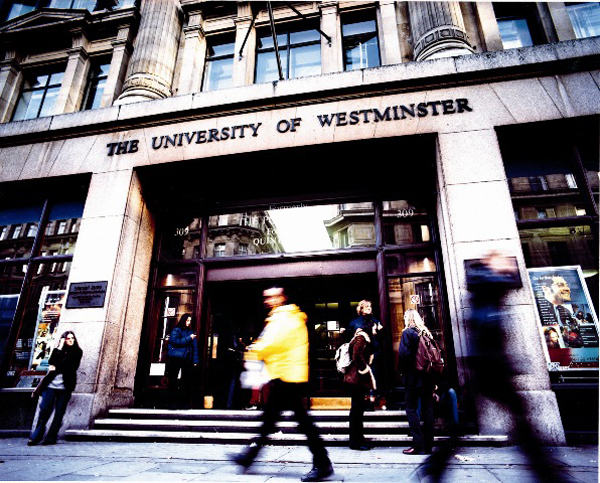
\includegraphics[scale=0.3]{westminsterRegentExterieur.jpg}}
	\qquad
	\subfloat[Entr\'ee]{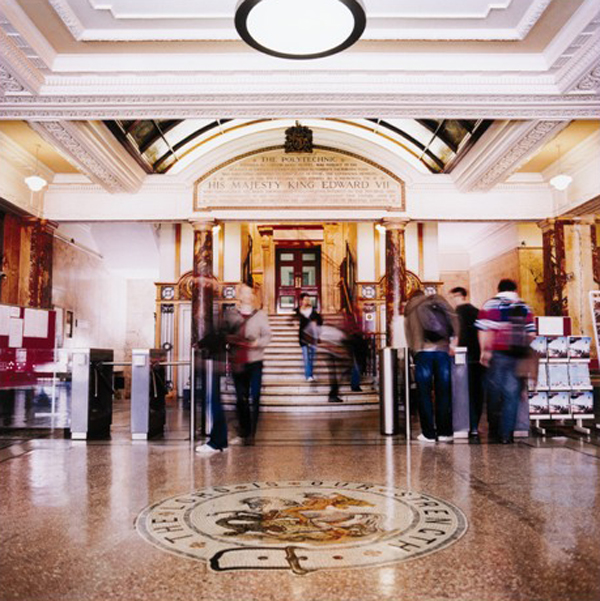
\includegraphics[scale=0.242]{westminsterRegentInterieur.jpg}}
	\caption{Campus de Regent Street}

\end{figure}

\noindent Outre ces principaux campus, l'universit\'e compte deux plus petits campus : 

\begin{itemize}
	\item \textbf{Little Tichtfield Street} : situ\'e au 4-12 Little Titchfield street, il contient une \'ecole : 
		\textit{School of Law};
	\item \textbf{Wells Street} : situ\'e au 32-38 Wells street, juste au coin des autres b\^atiments du campus de Regent, il offre une grande vari\'et\'e de salles de classe.

\end{itemize}

\vspace{0.20cm}

L'universit\'e g\`ere \'egalement le Westminster International University \`a Tachkent en Ouzb\'ekistan ainsi qu'un campus satellite \`a Paris \`a travers l'Acad\'emie Diplomatique de Londres.

\subsection{Quelques informations sur l'universit\'e}

L'universit\'e se situe officiellement au 309 Regent Street London W1B 2HM.
Elle compte en 2011 plus de 20 000 \'etudiants venant de plus de 150 nations diff\'erentes gr\^ace \`a de nombreux programmes d'\'echange avec d'autres universit\'es.

\noindent Parmi ses dipl\^om\'es les plus prestigieux :

\begin{itemize}
	\item Sir \textbf{Alexander Fleming}, biologiste et pharmacologue britannique, prix Nobel de Physiologie ou M\'ed\'ecine en 1945 avec Ernst Boris Chain et Sir Howard Walter Florey pour la d\'ecouverte de la p\'enicilline et de son effet curatif sur diverses maladies infectieuses;
	\item \textbf{Christopher Bailey}, directeur de la cr\'eation chez \textit{Burberry};
	\item \textbf{Charlie Watts}, musicien et batteur des \textit{Rolling Stones}.

\end{itemize}

\vspace{0.20cm}

\noindent Concernant les cours, l'universit\'e donne acc\`es \`a plus de 300 cours diff\'erents.

\section{School of Electronics and Computer Science}

Le stage s'est d\'eroul\'e dans cette \'ecole se trouvant, comme vu au \S~\ref{section:campus}, dans le campus Cavendish au 101-115 new Cavendish Street. 
La figure~\ref{figure:westminsterNewCavendish} montre une vue ext\'erieure du b\^atiment avec la BT Tower, tour de communication poss\'ed\'ee par l'op\'erateur de t\'el\'ecommunications BT Group, se trouvant juste \`a c\^ot\'e.

\begin{figure}[!ht]
	\centering
	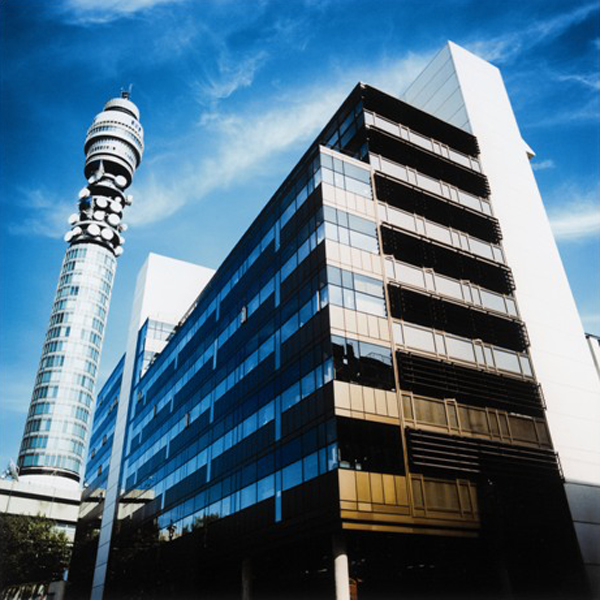
\includegraphics[scale=0.242]{westminsterNewCavendish.jpg}
	\caption{Campus de New Cavendish Street}
	\label{figure:westminsterNewCavendish}

\end{figure}

L'\'ecole propose divers parcours, aussi bien dans le domaine de la recherche que dans celui des \'etudes, allant de l'ing\'enierie \'electronique et informatique, aux math\'ematiques appliqu\'ees.
Ainsi de nombreuses mati\`eres peuvent \^etre abord\'ees dans la formation comme la gestion des syst\'emes d'informations, la programmation parall\`ele et distribu\'ee, l'intelligence artificielle mais aussi le d\'eveloppement de jeux vid\'eos et bien d'autres.

\noindent Il existe quatre grands p\^oles de recherche au sein de l'\'ecole qui sont :

\textit{Electronic and Communication Engineering}, qui se concentre sur le traitement de signaux ainsi que dans la conception de composants et circuits pour les syst\`emes de communication;

\textit{Operational Research and Intelligent Systems}, dont les activit\'es sont principalement la mod\'elisation quantitative des syst\`emes complexes pour soutenir des processus d\'ecisionnels, la gestion des donn\'ees et des informations, les technologies de base de donn\'ees destin\'ees au processus de gestion et d'interop\'erabilit\'e dans les environnements o\`u les logiciels sont omnipr\'esents;

\textit{Parallel and Distributed Computing}, qui s'int\'eresse \`a la recherche et au d\'eveloppement dans le domaine des calculs parall\`eles et distribu\'es;

\textit{Semantic Computing and Systems Engineering}, regroupe des chercheurs de diff\'erentes disciplines, comme le g\'enie logiciel, les interactions homme-machine, et aborde les aspects th\'eoriques et pratiques de l'informatique s\'emantique.

\section{\'Equipes int\'egr\'ees}

Le projet \YuukouII{} regroupe deux services de l'universit\'e. 
D'une part l'\textit{Infrastructure Team}, et d'autre part le \textit{Information Systems and Library Services} (ISLS).
Le but de mon stage \'etant de fournir un pilote de ce qu'il est possible de faire afin que mon travail puisse \^etre repris par les deux services et d\'evelopp\'e plus en profondeur.

\subsection{Infrastructure Team}

L'\textit{Infrastructure Team} est une \'equipe de 13 personnes dans la \textit{School of Electronics and Computer Science} qui a pour r\^ole de g\'erer les laboratoires sp\'ecialis\'es de l'\'ecole.
Ce sont 34 laboratoires de la facult\'e qui sont sous la responsabilit\'e de cette \'equipe.
Ces laboratoires sont dit sp\'ecialis\'es du fait des possibilit\'es qui peuvent \^etre r\'ealis\'ees : l'installation de nouveaux syst\`emes d'exploitations sur les ordinateurs par exemple.

L'\'equipe apporte aussi un support pour les laboratoires d'enseignement et pour les groupes de recherches dans la facult\'e.
Elle reprend et \'etend les services fournis par les services centraux informatique (voir ISLS au \S~\ref{section:ISLS}) comme l'authentification, les quotas de disques, le r\'eseau ou encore les outils d'enseignement.

\subsection{Information Systems and Library Services}
\label{section:ISLS}

ISLS est un d\'epartement dont le but est de contribuer \`a la qualit\'e de l'\'education dans l'universit\'e de Westminster \`a travers le d\'eveloppement et la livraison de services.

\noindent Le d\'epartement est compos\'e de cinq services qui sont :

\begin{itemize}
	\item Archive Services, qui g\`ere les enregistrements de l'universit\'e;
	\item Corporate Information, qui d\'eveloppe et livre des applications qui prennent en charge le fonctionnement des activit\'es (enregistrement des \'etudiants, emplois du temps, \ldots);
	\item Infrastructure, qui g\`ere l'infrastructure informatique pour fournir des services informatiques et de t\'el\'ecommunication;
	\item Learning and Research Support, qui g\`ere la biblioth\`eque et les services informatiques pour le personnel et les \'etudiants;
	\item Resources and Planning, qui g\`ere les ressources et le planning du d\'epartement.

\end{itemize}

\section{Centre for Parallel Computing}

Durant toute la dur\'ee de mon stage, j'ai travaill\'e dans le \textit{Centre for Parallel Computing} (CPC).
Le bureau se situe au 7\`eme \'etage de la \textit{School of Electronics and Computer Science} et est compos\'e de sept personnes.
Cette \'equipe appartient au p\^ole recherche \textit{Parallel and Distribued Computing}.

Ce centre se concentre sur la recherche dans la technologie et les applications de calculs parall\`eles et distribu\'ees.
Les activit\'es du cente incluent le d\'eveloppement d'outils et d'environnements pour soutenir le cycle de vie dans le g\'enie logiciel comme la simulation d'\'ev\'enements discrets en parall\`ele.
Les chercheurs travaillent en collaboration avec l'universit\'e hongroise Sztaki.

\noindent Parmi les projets d\'evelopp\'es par le service, on peut citer :

\begin{itemize}
	\item \textbf{Gemlca} (Grid Execution Management for Legacy Code Applications), solution g\'en\'erale dont le but est de deployer le code d'applications existantes, quelque soit le langage, comme un service de grille;
	\item \textbf{NGS} (National Grid Service), solution dont le but est de fournir un acc\`s \'electronique coh\'erent pour les chercheurs du Royaume-Uni \`a toutes les ressources de calculs et de donn\'ees ainsi qu'\`a l'\'equipement n\'ecessaire pour mener \`a bien leurs travaux, ind\'ependamment de l'emplacement de la ressource ou du chercheur;
	\item \textbf{SHIWA} (SHaring Interoperable Workflows for lages-scale scientific simulations on Available DCIs\protect\footnote{Distributed Computing Infrastructure}), projet qui a pour but l'interop\'erabilit\'e de diff\'erents syst\`emes de \textit{workflow}$^*$ europ\'een (comme Moteur, P-Grade, Askalon ou Gwes) avec l'aide de l'approche par granularit\'e (grain fin ou grossier).

\end{itemize}

\vspace{0.20cm}

Pendant le stage, j'ai \'et\'e rejoint par deux \'etudiants en troisi\`eme ann\'ee de licence informatique \`a l'universit\'e de Franche-Comt\'e de Besan\c{c}on : Yacine MAGHEZZI, travaillant sur la partie affichage du projet qui m'a \'et\'e confi\'e (plus d'explications au \S~\ref{section:architectureProjet}) et Damien HOSTACHE, travaillant sur le d\'eveloppement d'une application pour le portail Web de l'universit\'e de Westminster dans le but de g\'erer des objets en trois dimensions.


\clearpage


\chapter{Pr\'esentation du sujet}

\section{Le projet \Yuukou}

\begin{figure}[!ht]
	\centering
	
\includegraphics[scale=1]{yuukouLogo.jpg}

\end{figure}

\subsection{Pr\'esentation}

Le terme Yuukou comme abord\'e dans l'introduction de ce rapport, vient du japonais \Yuukou{} et signifie validit\'e, disponibilit\'e, efficacit\'e.
C'est un syst\`eme permettant la r\'ecup\'eration des informations depuis les serveurs LDAP\protect\footnote{\textit{Lightweight Directory Access Protocol}}$^*$ de l'Universit\'e afin de comprendre et construire l'infrastructure des ressources et ainsi de voir sa facilit\'e d'utilisation. 
L'architecture du syst\`eme utilise un processus d'apprentissage simple pour d\'eduire et maintenir la structure \`a jour avec un minimum de r\'eglages initiaux.
\Yuukou{} a \'et\'e cr\'e\'e pour montrer l'utilisation des salles informatiques et conserver un historique des informations sur le campus de New Cavendish.

\subsection{Fonctionnement}

Le but principal de \Yuukou{} est d'afficher l'occupation des salles informatiques en se rapprochant autant que possible du comportement d'un syst\`eme fonctionnant en temps r\'eel.
Pour ce faire, l'application a \'et\'e divis\'ee en deux parties  comme le montre la figure~\ref{figure:yuukouFonctionnement}.

\clearpage

\begin{figure}[!ht]
	\centering
	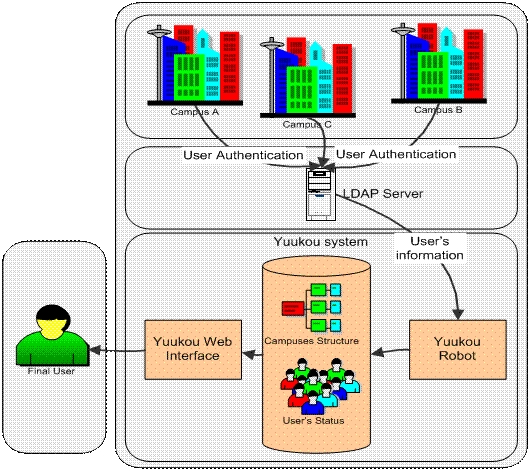
\includegraphics[scale=0.75]{yuukouFonctionnement.jpg}
	\caption{Architecture de \Yuukou}
	\label{figure:yuukouFonctionnement}

\end{figure}

\subsubsection{Premi\`ere partie}

La premi\`ere partie est un programme \'ecrit en Perl$^*$ qui r\'ecup\`ere les informations de connexion des utilisateurs depuis un serveur LDAP$^*$ et qui se charge de construire, modifier ou mettre \`a jour l'architecture r\'eseau de l'Universit\'e tout en stockant les informations dans une base de donn\'ees relationnelle de type MySQL.

Le robot de \Yuukou{} offre deux fonctionnalit\'es : il permet de mettre \`a jour les donn\'ees de connexion \textit{via} le serveur LDAP$^*$ toutes les cinq minutes environ pour une utilisation normale, et de mettre \`a jour le statut des ressources (ordinateurs) toutes les demi-heures, l\`a aussi pour une utilisation normale.

\subsubsection{Deuxi\`eme partie}

La seconde partie est un ensemble de pages Web \'ecrites en PHP\protect\footnote{\textit{Personal Home Page} ou \textit{PHP: Hypertext Preprocessor}}$^*$ et h\'eberg\'ees sur un serveur Web permettant de pr\'esenter les donn\'ees collect\'ees \`a l'utilisateur final.
Ces pages sont de deux types : les pages publiques et les pages priv\'ees.

Les pages publiques sont accessibles par tous les utilisateurs de l'Universit\'e le d\'esirant.
Les pages priv\'ees, quant \`a elles, ne sont accessibles qu'aux administrateurs.

\subsubsection{Les pages publiques}

\noindent Les pages publiques permettent l'affichage des pages suivantes :

\begin{itemize}
	\item une page contenant tous les campus et salles informatiques actuellement utilis\'ees;
	\item une page par campus avec les salles informatiques actuellement utilis\'ees;
	\item une page par campus et d\'epartement avec les salles informatiques actuellement utilis\'ees.

\end{itemize}

\vspace{0.20cm}

Les pages publiques offrent une vision g\'en\'erale de chaque salle : le nombre de ressources totales, disponibles, occup\'ees par un utilisateur et dans un \'etat inconnu.
Il est \`a noter que chacunes des pr\'ec\'edentes pages peut \^etre affich\'ees sur un \'ecran plasma pr\'esent dans les diff\'erents b\^atiments de l'Universit\'e.
La figure~\ref{figure:yuukouPublic} donne un exemple de page publique.

\subsubsection{Les pages priv\'ees}

\noindent Les pages priv\'ees permettent l'affichage des pages suivantes :

\begin{itemize}
	\item une page d'identification \textit{via} LDAP$^*$ pour l'administrateur;
	\item toutes les pages publiques mais b\'en\'eficiant de fonctionnalit\'es suppl\'ementaires :

	\begin{itemize}
		\item liste des ressources \'eteintes;
		\item une fen\^etre permettant d'avoir des informations sur un utilisateur actuellement connect\'e \`a une ressource (identifiant, nom, photo, heure de connexion et dur\'ee de la session);
		\item possibilit\'e d'ajouter des commentaires sur les utilisateurs;
		\item liens vers les statistiques des salles informatiques.

	\end{itemize}

\end{itemize}

\vspace{0.20cm}

La figure~\ref{figure:yuukouAdmin} donne un exemple des fonctionnalit\'es suppl\'ementaires auxquelles un administrateur a acc\`es.

\clearpage

\subsubsection{Vue sur le produit}

\begin{figure}[!ht]
	\centering
	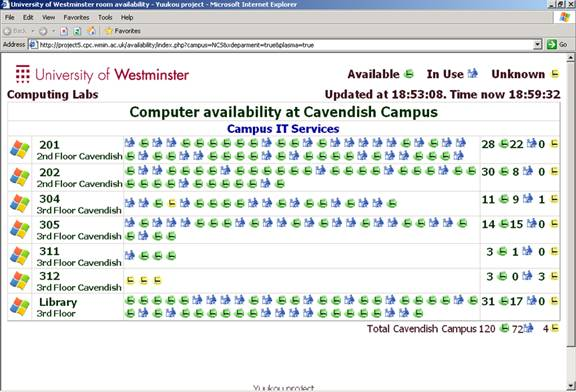
\includegraphics[scale=0.75]{yuukouPublic.jpg}
	\caption{Exemple de page publique de \Yuukou{} rep\'esentant un campus et l'utilisation des salles informatiques d'un d\'epartement}
	\label{figure:yuukouPublic}

\end{figure}

\begin{figure}[!ht]
	\centering
	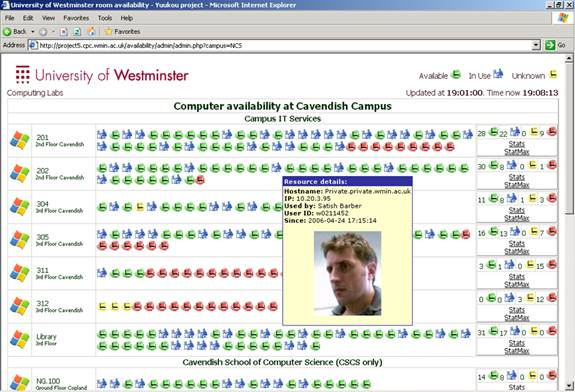
\includegraphics[scale=0.75]{yuukouAdmin.jpg}
	\caption{Exemple de page priv\'ee de \Yuukou{} montrant en particulier les donn\'ees d'un utilisateur}
	\label{figure:yuukouAdmin}

\end{figure}

\subsection{Quelques chiffres}

Le projet \Yuukou{} permet de surveiller le r\'eseau du campus de New Cavendish soit 43 salles informatiques, ce qui repr\'esente 661 PC. 
Le support des Macintosh n'\'etant pas pris en compte.

\subsection{Changement vers \YuukouII}

L'Universit\'e souhaite reprendre le principe du projet \Yuukou, cependant elle est confront\'ee \`a diff\'erents probl\`emes.
Le premier \'etant que les personnes ayant d\'evelopp\'e le projet ont quitt\'e l'Universit\'e. 
Ce qui signifierait, pour la personne ou l'\'equipe qui serait en charge de reprendre le projet, de prendre du temps pour se former \`a Perl$^*$, comprendre tout ce qui a \'et\'e d\'ej\`a r\'ealis\'e et ensuite seulement, commencer \`a d\'evelopper.
Actuellement de nombreux projets sont en cours et il n'est pas possible pour une \'equipe de passer du temps sur l'existant.

Un autre probl\`eme est les changements importants, du point de vue infrastructure, qui sont en train d'\^etre mis en place.
En effet, l'Universit\'e qui utilisait eDirectory$^*$ de Novell pour g\'erer ses annuaires LDAP$^*$ a commenc\'e \`a migrer toutes ses donn\'ees vers le syst\`eme Active Directory$^*$ de Microsoft qui est cens\'e \^etre plus efficace. Ce changement rendrait \Yuukou{} obsol\`ete.

Point suivant, la volont\'e de donner acc\`es aux informations sur les salles, pas seulement en utilisant un navigateur Internet, mais aussi et surtout en utilisant un \textit{smartphone} (IPhone ou autre par exemple) ou une tablette (IPad par exemple), chose que l'ancien logiciel ne peut pas fournir.
De ce fait, un \'etudiant aurait \`a tout moment les informations sur les salles \textit{via} son \textit{smartphone} ou sa tablette, si tant est qu'il ait l'un ou l'autre.

\noindent \`A ces pr\'ec\'edents probl\`emes, d'autres viennent s'ajouter :

\begin{itemize}
	\item les Macintosh ne sont pas pris en compte;
	\item le logiciel est assez monolithique, il deviendrait donc tr\`es difficile et complexe de vouloir l'\'etendre;
	\item {\Yuukou} ne prend en compte que les donn\'ees en temps r\'eel et ne garde pas un historique;
	\item son utilisation pr\^ete \`a confusion car il n'a aucun interfa\c{c}age avec l'emploi du temps, de ce fait, quand une salle est pr\'esent\'ee comme libre, il n'y a aucun moyen, avec le logiciel, de savoir si un cours s'y d\'eroule ou non.

\end{itemize}

\vspace{0.20cm}

C'est en consid\'erant tous ces points qu'il a \'et\'e d\'ecid\'e d'abandonner le projet \Yuukou{} afin de pouvoir mettre en place \YuukouII{} qui r\'epondrait aux attentes de l'Universit\'e.

\section{Le projet \YuukouII}

{\YuukouII} a pour but de combler les lacunes de {\Yuukou} et d'aller plus loin en termes de fonctionnalit\'es qu'il peut offrir. 
Le projet sera tout d'abord pr\'esent\'e avec les principaux points le composant.
Ensuite seront abord\'ees les diff\'erentes r\'eflexions que les \'equipes int\'eress\'es par le projet ont effectu\'ees.
Ces r\'eflexions donneront lieu aux premi\`eres id\'ees qui en ont \'emerg\'ees.
Enfin, les principales contraintes techniques du projet seront d\'ecrites.

\subsection{Pr\'esentation du projet}

Dans son fonctionnement g\'en\'eral, {\YuukouII} doit permettre de donner \`a un \'etudiant ou toute personne travaillant \`a l'Universit\'e et cherchant \`a utiliser un ordinateur, une vue globale des ressources qui sont disponibles actuellement.
Les donn\'ees devant \^etre bien s\^ur exactes afin que la personne n'ait pas de mauvaise surprise en se rendant dans une salle qu'elle pensait libre.
L'affichage pourra se faire \textit{via} un \textit{smartphone}, une tablette ou encore un navigateur Internet.

\noindent Le but du stage est : 

\begin{itemize}
	\item la conception d'un logiciel permettant la r\'ecup\'eration de donn\'ees concernant les connexions sur les diff\'erentes ressources de l'Universit\'e et cela en temps r\'eel;
	\item la gestion de la persistance de ces donn\'ees;
	\item la cr\'eation d'un maximum de fonctionnalit\'es retournant les informations utiles dans le but d'\^etre exploit\'ees pour l'affichage sur les diff\'erents supports.

\end{itemize} 

\vspace{0.20cm}

La cr\'eation d'applications permettant l'affichage des r\'esultats ne fait pas partie de ce sujet de stage. 
Ici, seule la partie r\'ecup\'eration, stockage et retour des donn\'ees est abord\'ee.

\subsection{R\'eflexions de l'\'equipe technique}

Diff\'erents acteurs de l'Universit\'e int\'eress\'es dans le projet \YuukouII{} ont commenc\'e \`a fixer une liste des fonctionnalit\'es qu'ils aimeraient voir avec l'application finale.

\subsubsection{Concernant les ressources}

\begin{itemize}
	\item Macintosh et Windows;
	\item conna\^itre l'\'etat de la ressource, \'eventuellement la d\'emarrer \`a distance (WOL\protect\footnote{\textit{Wake On Lan}}$^*$);
	\item inclure une surveillance partielle du mat\'eriel et des logiciels;
	\item utilisation des services d'Active Directory$^*$.

\end{itemize}

\subsubsection{Concernant les donn\'ees r\'ecup\'er\'ees}

\begin{itemize}
	\item mettre au point un formalisme avec les autres services de l'Universit\'e concernant les informations sur les salles, campus et d\'epartements;
	\item stocker les informations dans une base de donn\'ees SQL\protect\footnote{\textit{Structured Query Language}}$^*$;
	\item mettre en place des outils pour g\'en\'erer des statistiques \`a partir des donn\'ees stock\'ees (utilisation d'une salle, nombre de connexions par jour dans un mois pour une salle, \ldots).

\end{itemize}

\subsubsection{Concernant les donn\'ees retourn\'ees}

\begin{itemize}
	\item g\'en\'eration de flux RSS\protect\footnote{\textit{Rich Site Summary}}$^*$ pour retourner des informations;
	\item l'affichage doit \^etre en temps r\'eel et doit aussi permettre d'avoir une vue globale dans le temps : utilisation des emplois du temps pour savoir quelle salle est libre et \`a quel moment.

\end{itemize}

\vspace{0.20cm}

Cette liste n'est pas compl\`ete \'etant donn\'e qu'elle ne prend pas en compte la partie \og{}affichage\fg{} des r\'esultats du fait que le projet ne consiste qu'\`a la r\'ecup\'eration, au traitement et au retour de donn\'ees.

L'id\'ee initiale \'etait de d\'evelopper un projet pilote qui permettrait d'avoir une vue sur ce qu'il est possible de faire et sur la fa\c{c}on de le faire.
Il serait ensuite repris par les \'equipes de l'Universit\'e pour \^etre termin\'e.
Ce projet consisterait en la cr\'eation d'un service Web (la notion sera expliqu\'ee plus en d\'etail au \S~\ref{section:serviceWeb}) \'ecrit en C\# et utilisant le \textit{framework}$^*$ .Net de Microsoft.
Le service Web devra offrir un maximum de fonctionnalit\'es et \^etre exploit\'e par une application mobile pour \textit{smartphone} et par un site Web pouvant \^etre projet\'e sur les \'ecrans plasma \`a l'entr\'ee de chaque site.

Cependant, apr\`es r\'eflexion avec M. Thierry DELAITRE, la structure, les objectifs et le projet en g\'en\'eral ont \'et\'e revus.
Dans l'id\'ee initiale, pour conna\^itre l'\'etat d'une ressource, si elle est \'eteinte ou allum\'ee par exemple, il aurait fallu interroger Active Directory$^*$. 
De plus, n'est connu que l'\'etat si un utilisateur est connect\'e.
Il faudrait des traitements suppl\'ementaires pour pouvoir fixer pr\'ecisement l'\'etat d'une ressource, avec un \textit{ping} par exemple pour savoir si la ressource est \'eteinte ou non.

\subsection{Premi\`eres approches}

Une solution simple, rapide et fonctionnelle avait d\'ej\`a \'et\'e mise en place afin de \og{}monitorer\fg{}, \cad{} surveiller le fonctionnement des diff\'erentes ressources de certaines salles dans l'Universit\'e.
Nagios est une application permettant d'effectuer une surveillance syst\`eme et r\'eseau.
Il permet de conna\^itre l'\'etat d'une machine ainsi que d'autres informations comme le syst\`eme d'exploitation utilis\'e, la version de Java install\'ee, la charge du processeur, \ldots

En partant de ce logiciel, le projet consiste en la r\'ecup\'eration des donn\'ees de Nagios, leur traitement et le d\'eveloppement des fonctionnalit\'es permettant \`a une application ext\'erieure de pouvoir afficher les informations.

\noindent Les objectifs principaux deviennent les suivants :

\begin{itemize}
	\item cr\'eation d'un service Web en utilisant l'API\protect\footnote{\textit{Application Programming Interface}}$^*$ Java JAX-WS\protect\footnote{\textit{Java API for XML Web Services}};
	\item mise en place d'une m\'ethode de communication avec Nagios;
	\item cr\'eation de la base de donn\'ees permettant l'archivage;
	\item mise en place d'un cycle permettant de traiter les informations r\'ecup\'er\'ees;
	\item d\'efinition de fonctions utiles pour une application cliente;
	\item choix d'une structure de retour des informations pour une application cliente;
	\item faire un lien avec l'emploi du temps des diff\'erentes salles sous surveillance.

\end{itemize}

\subsection{Contraintes techniques}

Deux des principales contraintes du cahier des charges sont l'utilisation de logiciels libres et du langage de d\'eveloppement Java, tout en me laissant un maximum de libert\'e dans les autres choix.

Durant le stage, un ordinateur m'a \'et\'e fourni avec un libre choix sur le syst\`eme d'exploitation.
De ce fait j'ai opt\'e pour un Linux Mint 11 nomm\'e \textit{Katya}, que j'ai l'habitude d'utiliser.

Un autre ordinateur, lui contenant un Debian 6.0.5 nomm\'e \textit{Squeeze}, a \'et\'e mis \`a ma disposition en tant que serveur distant h\'ebergeant le service Web ainsi que les diff\'erents outils n\'ecessaires \`a son fonctionnement.
Le serveur distant contient le logiciel Nagios, le serveur Web permettant de faire fonctionner la derni\`ere version stable du service Web ainsi que le syst\`eme de gestion de bases de donn\'ees (SGBD).

Les tests \'etant en premier lieu r\'ealis\'es en local sur la machine de d\'eveloppement et ensuite, quand le fonctionnement \'etait garanti, l'application \'etait d\'eploy\'ee sur le serveur distant.
Des renseignements suppl\'ementaires seront apport\'es au \S~\ref{section:gestionProjet}.


\clearpage

\chapter{D\'ecouverte du projet}

\section{R\'eflexions de l'\'equipe technique}

Diff\'erents acteurs de l'universit\'e int\'eress\'es dans le projet \YuukouII{} ont commenc\'e \`a fixer une liste des fonctionnalit\'es qu'ils aimeraient voir avec l'application finale.

\subsubsection{Concernant les ressources}

\begin{itemize}
	\item Mac et Windows;
	\item conna\^itre l'\`etat de la ressource, \'eventuellement la d\'emarrer \`a distance (WOL\protect\footnote{\textit{Wake On Lan}}$^*$);
	\item inclure une surveillance partielle du mat\'eriel et des logiciels;
	\item utilisation des services de Active Directory$^*$.

\end{itemize}

\subsubsection{Concernant les donn\'ees r\'ecup\'er\'ees}

\begin{itemize}
	\item mettre au point un formalisme avec les diff\'erents autres services de l'universit\'e concernant les informations sur les salles, campus et d\'epartements;
	\item stocker les informations dans une base de donn\'ees SQL\protect\footnote{\textit{Structured Query Language}}$^*$;
	\item mettre en place des outils pour g\'en\'erer des statistiques \`a partir des donn\'ees stock\'ees (utilisation d'une salle, nombre de connexion par jour dans un mois pour un salle, \ldots).

\end{itemize}

\subsubsection{Concernant les donn\'ees retourn\'ees}

\begin{itemize}
	\item g\'en\'eration de flux RSS\protect\footnote{\textit{Rich Site Summary}}$^*$ pour retourner des informations;
	\item l'affichage doit \^etre en temps r\'eel et doit aussi permettre d'avoir un vue globale dans le temps : utilisation des emplois du temps pour savoir quelle salle est libre \`a quel moment.

\end{itemize}

\vspace{0.20cm}

Cette liste n'est pas compl\`ete du fait qu'elle ne prend pas en compte la partie \og{}affichage\fg{} des r\'esultats du fait que le projet ne consiste qu'\`a la r\'ecup\'eration, au traitement et au retour de donn\'ees.

L'id\'ee initiale \'etait de d\'evelopper un projet pilote qui permettrait d'avoir une vue sur ce qu'il est possible de faire et de la fa\c{c}on de le faire.
Il serait ensuite repris par les \'equipes de l'universit\'e pour \^etre termin\'e.
Ce projet consisterait en la cr\'eation d'un service Web$^*$ (la notion sera expliqu\'ee plus en d\'etail au \S~\ref{section:serviceWeb}) \'ecrit en C\# et utilisant le framework$^*$ .Net de Microsoft.
Le service Web devrait offrir un maximum de fonctionnalit\'es et devra \^etre exploit\'e par une application mobile pour \textit{smartphone} et par un site web pouvant \^etre projet\'e sur les \'ecrans plasma \`a l'entr\'e de chaque site.

Cependant, apr\`es r\'eflexion avec M. Thierry DELAITRE, la structure, les objectifs et le projet en g\'en\'eral ont \'et\'e revus.
Dans l'id\'ee initiale, pour conna\^itre l'\'etat d'une ressource, il aurait fallu interroger Active Directory$^*$. 
De plus, n'est connu que l'\'etat si un utilisateur est connect\'e.
Il faudrait des traitements suppl\'ementaires pour pouvoir fixer pr\'ecisement l'\'etat d'une ressource, avec un \textit{ping} par exemple.

\section{Premi\`eres approches}

Une solution simple, rapide et fonctionnelle avait d\'ej\`a \'et\'e mise en place afin de \og{}monitorer\fg{}, \cad{} surveiller le fonctionnement des diff\'erentes ressources de certaines salles dans l'universit\'e.
Nagios est une application permettant d'effetuer une surveillance syst\`eme et r\'eseau.
Il permet de conna\^itre l'\'etat d'une machine ainsi que d'autres informations comme le syst\`eme d'exploitation utilis\'e, la version de Java install\'ee, la charge du processeur, \ldots

En partant de ce logiciel, le projet consiste en la r\'ecup\'eration des donn\'ees de Nagios, leur traitement et le d\'eveloppement des fonctionnalit\'es permettant \`a une application ext\'erieure de pouvoir afficher les informations.

\noindent Les objectifs principaux deviennent les suivants :

\begin{itemize}
	\item cr\'eation d'un service Web en utilisant l'API\protect\footnote{\textit{Application Programming Interface}}$^*$ Java JAX-WS\protect\footnote{\textit{Java API for XML Web Services}};
	\item mise en place d'une m\'ethode de communication avec Nagios;
	\item cr\'eation de la base de donn\'ees permettant l'archivage;
	\item mise en place d'un cycle permettant de traiter les informations r\'ecup\'er\'ees;
	\item d\'efinition de fonctions utiles pour une application cliente;
	\item choix d'une structure de retour des informations pour une application cliente;
	\item faire un lien avec l'emploi du temps des diff\'erentes salles sous surveillance;

\end{itemize}

\section{Contraintes techniques}

Deux des principales contraintes du cahier des charges sont l'utilisation de logiciels libres et du langage de d\'eveloppement Java, tout en me laissant un maximum de libert\'e dans les autres choix.

Durant le stage, un ordinateur m'a \'et\'e fourni avec libre choix sur le syst\`eme d'exploitation.
De ce fait j'ai opt\'e pour un Linux Mint 11 nomm\'e \textit{Katya}, que j'ai l'habitude d'utiliser.

Un autre ordinateur, lui contenant un Debian 6.0.5 nomm\'e \textit{Squeeze}, a \'et\'e mis \`a ma disposition en tant que serveur distant h\'ebergeant le service Web ainsi que les diff\'erents les outils n\'ecessaires \`a son fonctionnement.
Le serveur distant contient le logiciel Nagios, le serveur Web permettant de faire fonctionner la derni\`ere version stable du service Web ainsi que le syst\`eme de gestion de base de donn\'ees (SGBD).

Les tests \'etant en premier lieu r\'ealis\'es en local sur la machine de d\'eveloppement et ensuite, quand le fonctionnement \'etait garanti, l'application \'etait d\'eploy\'ee sur le serveur distant.
Des renseignements suppl\'ementaires seront apport\'es au \S~\ref{section:gestionProjet}.



\clearpage


\chapter{Le projet Yuukou II}

Une fois le sujet pos\'e et la notion de service Web comprise, plusieurs recherches ont \'et\'e n\'ecessaires afin de pouvoir commencer le projet en lui-m\^eme.
C'est seulement ensuite que la phase de d\'eveloppement a pu commencer.
Le premier point traitera de la phase de recherche sur les outils et les choix qui ont \'et\'e pris pour le projet.
Ensuite un second point abordera la m\'ethode utilis\'ee pour acc\`eder aux informations indispensables au fonctionnement du service Web.
Les deux points suivant seront consacr\'es au fonctionnement et aux fonctionnalit\'e qu'offre le service Web.
Le premier de ces deux points permettra de d\'ecouvrir le cycle qui permet de r\'ecup\'erer les informations de Nagios et des les archiver, le deuxi\`eme, les m\'ethodes auxquelles un client peut acc\'eder pour r\'ecup\'erer une partie ou toutes les informations archiv\'ees par le service Web.
Suite \`a cela, un point aura pour but d'expliquer l'organisation du travail qui a \'et\'e adopt\'ee tout au long du d\'eveloppement du service Web.
Une vue sur comment est exploit\'ee le service Web sera faite ensuite et montrera des captures d'\'ecran de ce qui a \'et\'e r\'ealis\'e.
Enfin, un dernier point permettra de voir les principaux probl\`emes qui ont \'et\'e rencontr\'es lors du stage.

%%%%%%%%%%%%%%%%%%%%%%%%%%%
% RECHERCHES %%%%%%%%%%%%%%
%%%%%%%%%%%%%%%%%%%%%%%%%%%
\section{Recherches}

Une fois la notion de service Web acquise, il a fallu se concentrer sur la fa\c{c}on et les diff\'erents outils \`a utiliser afin de d\'evelopper le projet.
La r\'eflexion se portera d'abord sur une architecture du projet dont le but est de se faire une id\'ee de comment toutes les pi\`eces peuvent s'articuler les unes avec les autres.
Ensuite il sera fait une description des outils utilis\'es durant le projet.
Enfin les choix techniques pris lors du stage seront d\'ecrit.

\subsection{Architecture du projet}
\label{section:architectureProjet}

Le premier travail a \'et\'e la r\'eflexion sur comment mettre en place une solution pouvant communiquer avec Nagios dont une description sera faite au \S~\ref{section:nagios}.
Les figures~\ref{figure:architectureProjetServiceWeb} et~\ref{figure:architectureProjetAffichage} pr\'esentent le fruit des recherches qui ont \'et\'e faites sur la mise en place du projet \YuukouII.

\begin{figure}[!ht]
	\centering
	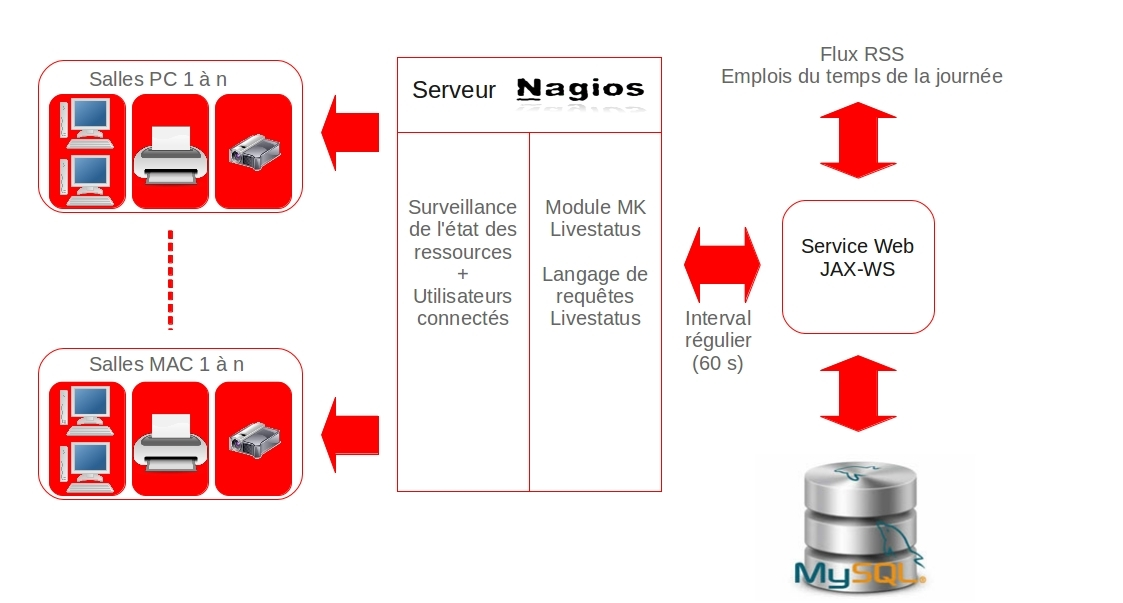
\includegraphics[scale=0.35]{architectureProjetServiceWeb.jpg}
	\caption{Architecture du projet, partie service Web}
	\label{figure:architectureProjetServiceWeb}

\end{figure}

\begin{figure}[!ht]
	\centering
	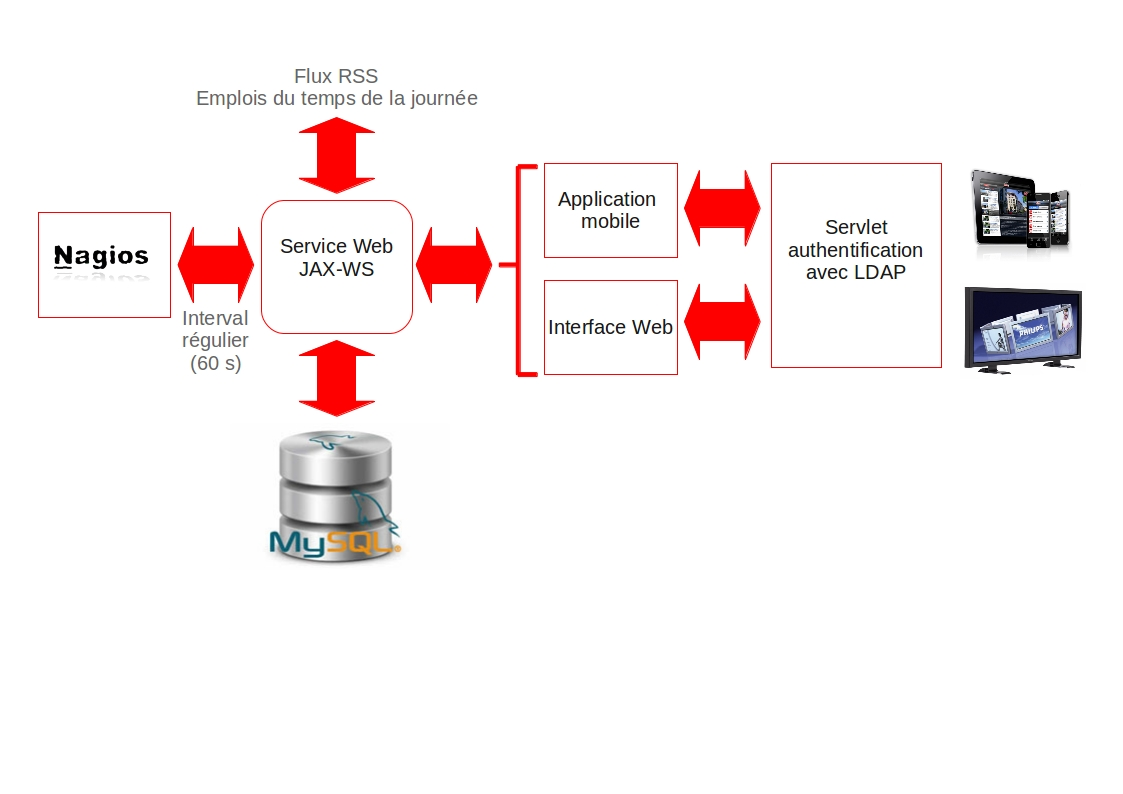
\includegraphics[scale=0.35]{architectureProjetAffichage.jpg}
	\caption{Architecture du projet, partie affichage}
	\label{figure:architectureProjetAffichage}

\end{figure}

\subsubsection{Partie service Web}

Basiquement Nagios sert \`a surveiller les ressources auxquelles il lui est permis d'acc\'eder.
De ce fait, il doit garder des traces des informations qu'il r\'ecup\`ere.
Ces informations sont stock\'ees dans un fichier.
C'est pourquoi un module existe sp\'ecialement pour acc\'eder aux informations contenues dans ce fichier. 
Le module \textit{MK Livestatus} permet \`a l'aide d'un langage de requ\^etes qui lui est propre, de r\'ecup\'erer les informations que garde Nagios.

Le service Web doit permettre, dans un premier temps, de r\'ecup\'erer toutes les informations utiles pour un archivage des donn\'ees.
Elles sont stock\'ees dans une base de donn\'ees MySQL.
\noindent Ces informations sont :

\begin{itemize}
	\item les donn\'ees r\'ecup\'er\'ees via le module \textit{MK Livestatus}, la r\'ecup\'eration doit \^etre faite \`a intervalles r\'eguliers;
	\item les diff\'erents emplois du temps de toutes les salles que Nagios surveille, la r\'ecup\'eration doit \^etre faite une fois par jour;
	\item les donn\'ees sur un utilisateur inconnu (nom, pr\'enom, r\^ole : \'etudiant par exemple, photo) via un serveur LDAP.

\end{itemize}

\subsubsection{Partie affichage}

Dans un deuxi\`eme temps, le service Web doit pouvoir retourner ces informations tri\'ees \`a un utilisateur normal ou un administrateur afin de garantir l'affichage sous la forme d'une application mobile ou d'une interface Web.
La r\'eflexion doit ainsi se porter sur le contenu des diff\'erentes m\'ethodes auxquelles un utilisateur pourra avoir acc\`es (en fonction qu'il soit administrateur ou non).
Le but \'etant un affichage le plus rapide possible des informations demand\'ees.

L'utilisateur doit s'authentifier via un \textit{Servlet}$^*$ qui communique avec LDAP$^*$ et qui donne un acc\`es \`a l'application.
Le reste de la communication est s\'ecuris\'ee comme expliqu\'e dans le \S~\ref{section:securisation}.

Le dernier point est de choisir un format pour les donn\'ees qui seront \'echang\'ees entre le service Web et l'application cliente.
C'est sur cette partie que Yacine MAGHEZZI est intervenu durant son stage.

\subsection{Nagios}
\label{section:nagios}

\begin{figure}[!ht]
	\centering
	
\includegraphics[scale=0.5]{nagiosLogo.jpg}
	\caption{Logo de Nagios}

\end{figure}

\subsubsection{Pr\'esentation}

Nagios est une application permettant la surveillance syst\`eme et r\'eseau de toute une infrastructure informatique.
Nagios compl\`ete cette surveillance en offrant la possibilit\'e d'alerter les \'equipes en charge de l'infrastructure en cas d'apparition de probl\`emes comme une panne ou encore un fonctionnement anormal.
C'est actuellement la solution de surveillance la plus efficace du march\'e.

\parpic{
	\begin{minipage}{0.20\textwidth}
		
\includegraphics[scale=0.6]{netsaintLogo.jpg}
	\end{minipage}}
Nagios a \'et\'e cr\'e\'e en 1999 et portait initialement le nom de \textit{NetSaint Network Monitor}.
Il est \'ecrit en C et est con\c{c}u pour un environnement Unix.
Le projet a \'et\'e maintenu jusqu'en 2002 avant de changer de nom pour devenir Nagios en r\'eponse \`a une contestation judiciaire par les propri\'etaires d'une marque similaire.
N.A.G.I.O.S. est l'acronyme r\'ecursif de \og{}\textit{Nagios Ain't Gonna Insist On Sainthood}\fg{} o\`u Sainthood est une r\'ef\'erence \`a \textit{NetSaint}.

Maintenant connu sous le nom de Nagios XI, Nagios est un logiciel libre sous la licence GNU GPL V2. 
Il est disponible sur son site Internet\cite{biblio:siteNagios} en version 3.2.1.

\subsubsection{Fonctionnement}

\noindent L'architecture de base de Nagios est tr\`es simple, elle comporte :

\begin{itemize}
	\item un ordonnanceur pour g\'erer les v\'erifications ainsi que les actions \`a prendre sur les diff\'erents incidents;
	\item une partie graphique : visible \`a travers un simple serveur Web;
	\item des sondes : greffons (ou \textit{plugins} en anglais) dans Nagios, ce sont de petits \textit{scripts} permettant d'effectuer diverses v\'erifications.

\end{itemize}

\vspace{0.20cm}

\`A la base, Nagios est un moteur d'ordonnancement de v\'erifications diverses et vari\'ees dont les v\'erifications sont effectu\'ees via des greffons.
Ces v\'erifications peuvent \^etre la charge d'utilisation du CPU\protect\footnote{\textit{Central Processing Unit} ou processeur en fran\c{c}ais}, l'espace disque utilis\'e ou encore qui est connect\'e actuellement.
Dans le cadre de la v\'erification de l'infrastructure, deux types de machines sont observ\'ees : les ordinateurs dot\'es de Windows et les ordinateurs dot\'es de Macintosh.

Nagios \'etant install\'e et fonctionnel depuis un peu plus d'un an sur le site de New Cavendish, les greffons pour observer les deux types de machines ont d\'ej\`a \'et\'e d\'evelopp\'es.
Pour les machines fonctionnant sous Windows, le greffon est en fait l'appel \`a la commande Unix \textit{Winexe} qui permet l'ex\'ecution de commandes \`a distance sur des machines Windows.
Pour les machines fonctionnant sous Macintosh, le greffon effectue une connexion SSH\protect\footnote{\textit{SecureShell}}, offrant une connexion s\'ecuris\'ee sur une machine distante pour ensuite ex\'ecuter la commande Unix \textit{who} permettant l'obtention de l'utilisateur connect\'e.
Pour les machines b\'en\'eficiant d'un double \textit{boot} (d'un d\'emarrage de l'ordinateur permettant de choisir entre deux syst\`emes d'exploitation) Windows-Unix, seul le syst\`eme Windows est surveill\'e.
La configuration actuelle de Nagios ne permet pas de r\'ecup\'erer avec exactitude l'utilisateur connect\'e sur le syst\`eme Unix.
Il est juste possible de savoir que l'ordinateur est occup\'e, mais pas par qui.

La configuration de Nagios s'articule entre diff\'erents concepts : les \textit{hosts}, les \textit{hostgroups} les \textit{services}.
Un \textit{host} repr\'esente un ordinateur, cet ordinateur poss\`ede des \textit{services} comme le service \textsf{check\_whoisloggedin} permettant de savoir si un utilisateur est actuellement connect\'e sur ladite machine.
Il faut enfin partie d'un groupe d'ordinateurs \textit{hostgroups} qui repr\'esente une salle informatique au sein de l'Universit\'e.

\subsubsection{\og{}\textit{Monitoring}\fg{} \`a l'Universit\'e}

Initialement, Nagios surveillait juste les machines se situant sur le campus de New Cavendish, soit 31 salles PC seulement machines.
Actuellement, ce sont 102 salles qui sont sous la surveillance de Nagios, soit 99 salles utilisant Windows soit 1920 PC, 3 salles utilisant des Macintosh soit 63 MAC, pour un total de 1983 machines \`a travers toute l'Universit\'e : la grande majorit\'e des ordinateurs de l'Universit\'e.
Il faut noter que seuls les Macintosh de New Cavendish sont sous surveillance, les autres n\'ecessitant d'\^etre list\'es et des acc\`es diff\'erents.
De ce fait, le nombre de machines devrait augmenter par la suite.

\subsubsection{Vue sur la surveillance de Nagios}

Les figures~\ref{figure:nagiosGeneral} et~\ref{figure:nagiosCG24}  donnent un aper\c{c}u de l'interface graphique de configuration mais aussi de suivi de Nagios.
La figure~\ref{figure:nagiosGeneral} offre une vue d'ensemble sur tous les  \textit{hosts} de tous les \textit{hostgroups} surveill\'es.
La figure~\ref{figure:nagiosCG24}, quant \`a elle, offre une vue pour un \textit{hostgroup} sp\'ecifique : la salle pourtant le nom \textsf{e-cg24}.

\clearpage

\begin{figure}[!ht]
	\centering
	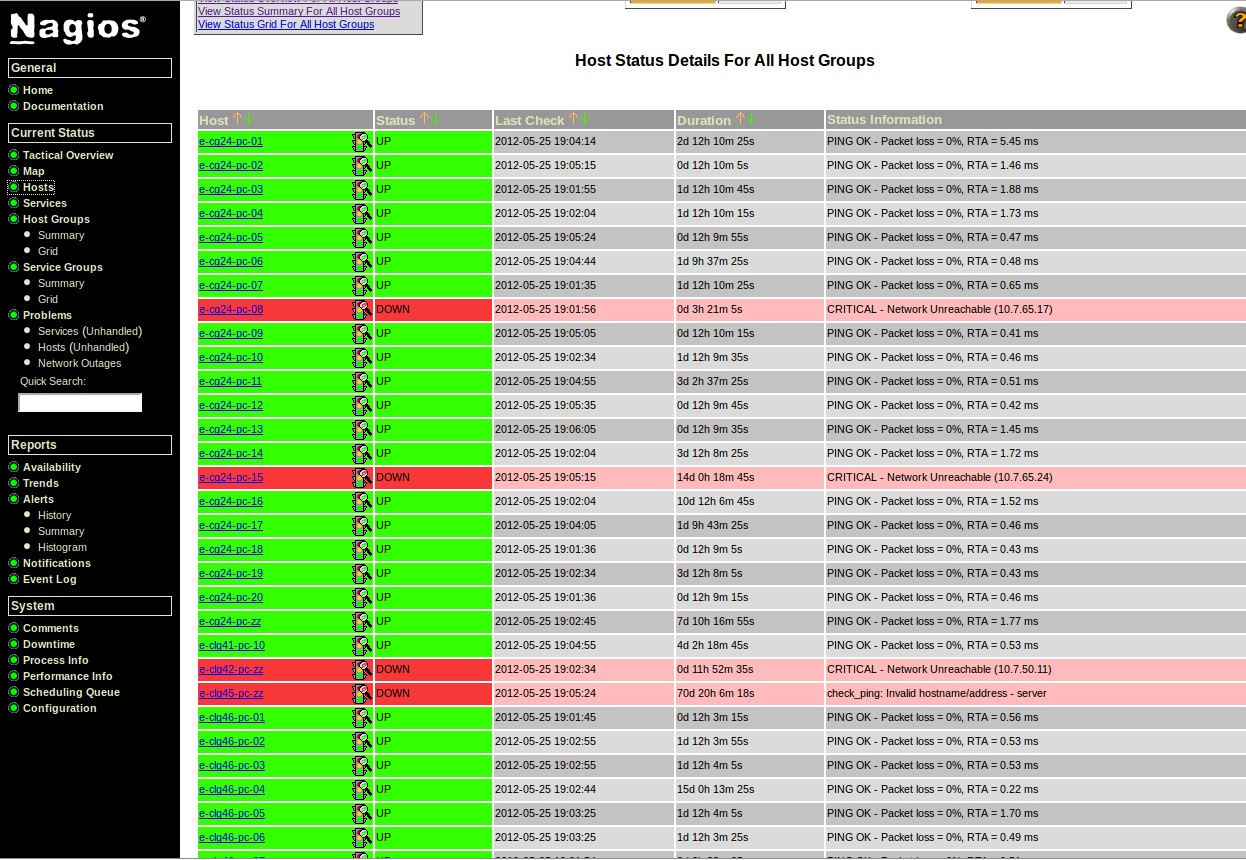
\includegraphics[scale=0.375]{nagiosGeneral.jpg}
	\caption{Exemple d'affichage de Nagios, vue sur tous les \textit{hostgroups}}
	\label{figure:nagiosGeneral}
	
\end{figure}

\begin{figure}[!ht]
	\centering
	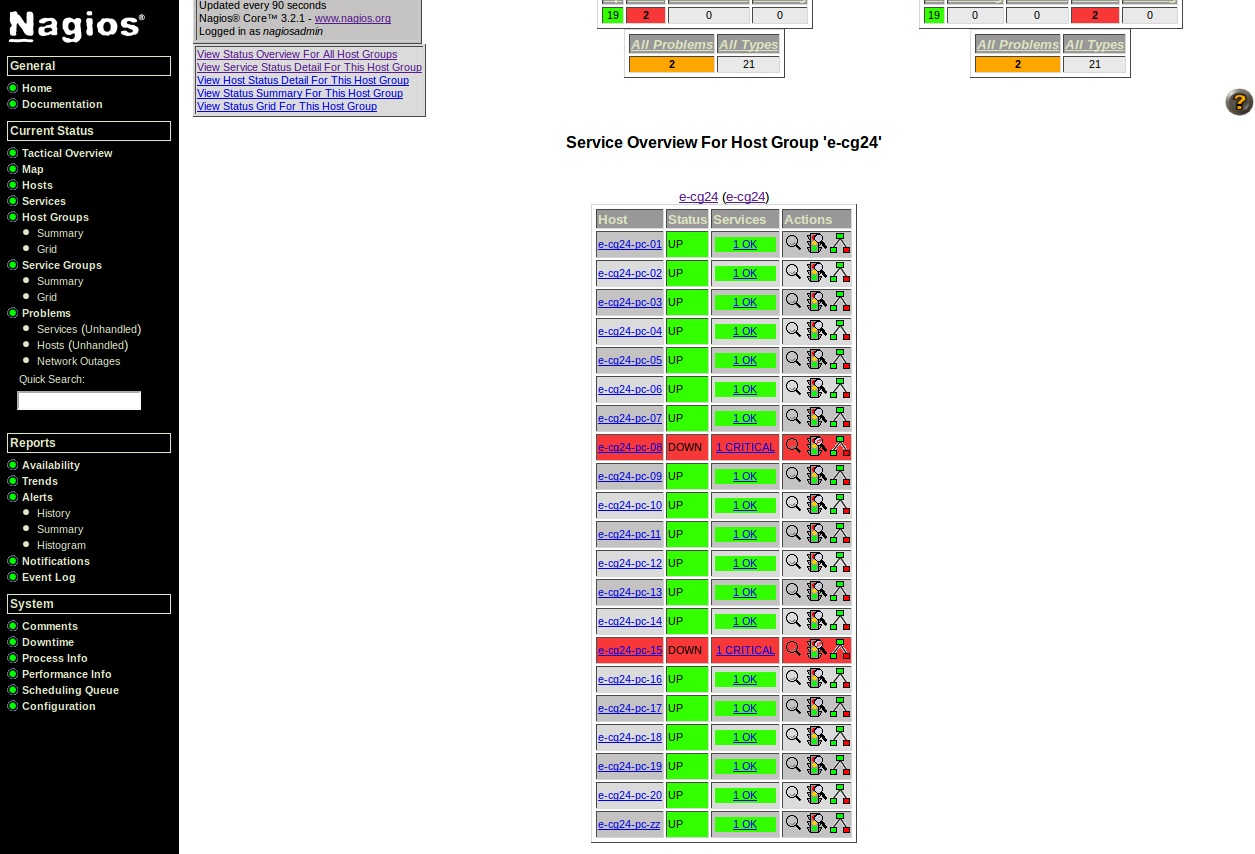
\includegraphics[scale=0.375]{nagiosCG24.jpg}
	\caption{Exemple d'affichage de Nagios, vue sur tous les \textit{hosts} d'un \textit{hostgroup} sp\'ecifique}
	\label{figure:nagiosCG24}
	
\end{figure}

\subsection{L'IDE NetBeans}
\label{section:netbeans}

\begin{figure}[!ht]
	\centering
	
\includegraphics[scale=0.25]{netbeansLogo.jpg}
	\caption{Logo de NetBeans}

\end{figure}

NetBeans est un IDE\protect\footnote{\textit{Integrated Development Environment}}$^*$ \textit{open source} d\'evelopp\'e par Sun Microsystems permettant le d\'eveloppement en utilisant les langages de programmation tels que Java, JavaScript, PHP$^*$, C, C++, et autres.
Il est \'ecrit en Java et fonctionne sous Windows, Mac OS, Linux, Solaris et d'autres plates-formes du moment qu'elles poss\`edent une JVM\protect\footnote{\textit{Java Virtual Machine}}$^*$ compatible.

NetBeans permet de d\'evelopper et d\'eployer rapidement des applications graphiques Swing, des Applets, des JSP/Servlets et des architectures J2EE\protect\footnote{\textit{Java Platform, Enterprise Edition}}.
Il poss\`ede toutes les fonctionnalit\'es recherch\'ees dans un IDE$^*$ moderne (coloration syntaxique, refactoring, d\'ebogueur, \ldots) et ajoute, dans le cas d'un d\'eveloppement d'un service Web comme pour ce projet, un support avec la derni\`ere version de GlassFish, permettant notamment de faire des {\og}deploy on save{\fg}, de d\'eployer les applications Web sur un serveur distant et de contr\^oler le serveur (suivre la sortie de logs, d\'emarrer, arr\^eter le serveur). 
Il donne acc\`es \`a une gestion simple du serveur d'application GlassFish qui sera utilis\'e dans le projet.
Sa premi\`ere version date de 1996 et portait le nom Xelfi. 
Il est disponible sur son site Internet\cite{biblio:siteNetbeans} en version 7.1.2.

\subsection{Le serveur Web GlassFish}
\label{section:glassfish}

\begin{figure}[!ht]
	\centering
	
\includegraphics[scale=0.35]{glassfishLogo.jpg}
	\caption{Logo de GlassFish}

\end{figure}

GlassFish est un serveur d'application \textit{open source} d\'evelopp\'e par Sun Microsystems pour les plates-formes Java EE\protect\footnote{\textit{Java Platform, Entreprise Edition}} 5 et 6, et est maintenant maintenu par Oracle Corporation.
Il dispose de nombreux outils pour faciliter le d\'eveloppement, le d\'eploiement et la maintenance d'application.
Un de ses avantages est qu'il est particuli\`erement bien int\'egr\'e \`a NetBeans, ce qui permet un d\'eploiement tr\`es rapide des applications ainsi qu'une trace d'ex\'ecution lors du fonctionnement.
GlassFish est disponible sur son site Internet\cite{biblio:siteGlassfish} en version 3.1.2.

\subsection{Le SGBD MySQL}

Un des objectifs du projet {\YuukouII} est un archivage temporel des donn\'ees.
Le but \'etant de g\'en\'erer des statistiques d'utilisation des salles informatiques des diff\'erents campus par exemple.

\begin{figure}[!ht]
	\centering
	
\includegraphics[scale=0.75]{mysqlLogo.jpg}
	\caption{Logo de MySQL}
	
\end{figure}

MySQL est le Syst\`eme de Gestion de Base de Donn\'ees (SGBD) la plus populaire qui fonctionne comme un serveur fournissant un acc\`es multi-utilisateurs \`a des bases de donn\'ees de type SQL$^*$.
Il a \'et\'e cr\'e\'e par MySQL AB en 1995, rachet\'e par Sun Microsystems et est maintenant maintenu par Oracle.
Il pr\'esente les avantages d'\^etre \textit{open source}, gratuit, fiable, rapide et facile \`a utiliser.
Il est tr\`es souvent utilis\'e avec le langage de cr\'eation de pages Web dynamique PHP$^*$.
C'est donc avec cet outil que les donn\'ees de {\YuukouII} seront archiv\'ees.
MySQL est disponible sur son site Internet\cite{biblio:siteMySQL} en version 5.5.24.

\subsection{L'acc\`es aux donn\'ees des tables}

Par souci de performance, \cad, limiter les acc\`es multiples \`a la base de donn\'ees mais aussi faciliter la manipulation des donn\'ees lors des traitements, le design pattern$^*$ \textit{Data Access Object} (DAO) a \'et\'e utilis\'e.
Un Data Access Object, ou objet d'acc\`es aux donn\'ees en fran\c{c}ais, est un objet qui constitue une repr\'esentation en m\'emoire des donn\'ees d'une base de donn\'ees.
En Java, un DAO est une classe repr\'esentant une table dont les attributs sont les champs de la table comme le montre la figure~\ref{figure:dao}.
Des classes repr\'esentant des listes sont g\'en\'eralement d\'evelopp\'ees pour contenir les DAO et simplifier l'acc\`es aux donn\'ees.

Lorsqu'il sera n\'ecessaire d'effectuer des traitements r\'ep\'et\'es sur les donn\'ees d'une table, m\^eme si ces traitements ne portent pas sur la totalit\'e de la table, il est pr\'ef\'erable de charger en m\'emoire la totalit\'e des \'el\'ements utiles avec, dans le cas id\'eal, une seule requ\^ete SQL$^*$.

\begin{figure}[!ht]
	\centering
	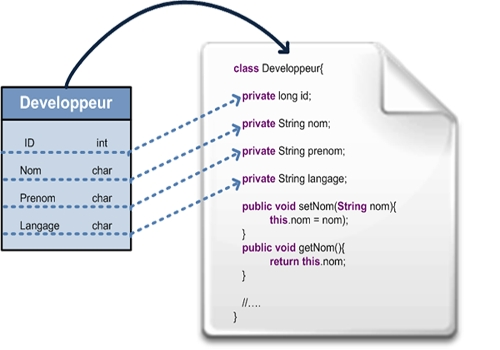
\includegraphics[scale=0.5]{dao.jpg}
	\caption{Exemple de \textit{mapping} d'une table avec sa classe DAO associ\'ee (\textit{source : Cyrille Herby})}
	\label{figure:dao}

\end{figure}

Dans le cadre du projet, les chargements sont effectu\'es lorsqu'un client appelle une m\'ethode du service Web. 
Les donn\'ees sont charg\'ees dans une liste, elles sont ensuite trait\'ees puis retourn\'ees au client.

\subsection{Le format de retour}
\label{section:formatRetour}

Le choix du type de retour est un choix important.
En effet, il faut que les donn\'ees puissent \^etre rapidement transmises, r\'ecup\'er\'ees, trait\'ees et affich\'ees.
L'objectif est un affichage instantan\'e des pages sur le navigateur Web ou l'application mobile.
De ce fait, plusieurs possibilit\'es ont \'et\'e envisag\'ees.

\subsubsection{{\og}\textit{Parsing}{\fg} d'un texte}

La premi\`ere est de transmettre un document texte basique, celui-ci format\'e d'une certaine fa\c{c}on afin d'\^etre \textit{pars\'e} ({\cad} parcourir un flux structur\'e d'informations pour en extraire les donn\'ees).
Ce qui aurait comme avantage de pouvoir \^etre r\'ecup\'er\'e par un client utilisant n'importe quel langage.
La figure~\ref{code:exemplePlaintext} repr\'esente un exemple de fichier qu'il est facile de \textit{parser}, il suffit de r\'ecup\'erer les informations se trouvant entre les arobases.

\clearpage

\begin{figure}[!ht]
	\begin{lstlisting}[language=plaintext]
info1 @ info2 @ info3 @ info4
	\end{lstlisting}
	
	\caption{Exemple de ligne pouvant \^etre facilement \textit{pars\'ee}}
	\label{code:exemplePlaintext}

\end{figure}

Pour r\'ecup\'erer les informations de cet exemple, il suffit de parcourir le fichier en stockant les informations contenues entre les \textbf{@}.

Cependant cette m\'ethode est assez contraignante et oblige \`a parcourir l'ensemble du fichier alors qu'un seul type d'information peut \^etre utile.
Ce qui signifie une perte de temps plus ou moins significative en fonction de la taille du fichier re\c{c}u.

\subsubsection{Objet Java s\'erialisable}

Une autre m\'ethode pourrait \^etre de transmettre un objet Java dit s\'erialisable.
La s\'erialisation est un m\'ecanisme fourni par Java permettant de consid\'erer un objet comme une s\'equence de d'octets qui inclut les donn\'ees de l'objet, le type de l'objet et le type des donn\'ees.
De cette mani\`ere, l'objet en question peut \^etre transmis \`a travers le r\'eseau vers une autre application Java pour le r\'ecup\'erer et le d\'es\'erialiser, ce qui repr\'esente la proc\'edure inverse de la s\'erialisation.
La figure~\ref{code:exempleJava} donne un exemple de classe Java s\'erialisable qui pourrait \^etre transmise par le r\'eseau comme un flux de bytes.

\vspace{0.20cm}

\begin{figure}[!ht]
	\lstinputlisting[language=Java]{codes/Exemple.java}
	\caption{Exemple de classe Java s\'erialisable}
	\label{code:exempleJava}

\end{figure}

L'objet contiendrait toutes les donn\'ees utiles et celles-ci seraient facilement accessibles.
Le probl\`eme venant avec cette solution est que les objets doivent \^etre r\'ecup\'er\'es par une JVM$^*$.
Ce qui peut s'av\'erer plus ou moins compliqu\'e voir impossible dans d'autres langages de programmation que Java.

\subsubsection{XML}

eXtensible Markup Language ou XML est un m\'eta langage pour r\'ealiser du balisage g\'en\'erique permettant de mettre en forme les documents. XML a connu un grand succ\`es depuis sa cr\'eation.
Il est utilis\'e en particulier pour g\'erer la configuration, le stockage des donn\'ees, l'\'echange d'informations et bien d'autres fonctions encore.
La figure~\ref{code:exempleXML} donne un exemple de document XML pouvant \^etre facilement converti en une arborescence DOM$^*$.

\vspace{0.20cm}

\begin{figure}[!ht]
	\lstinputlisting[language=XML]{codes/Exemple.xml}
	\caption{Exemple de document XML}
	\label{code:exempleXML}

\end{figure}

XML offre une solution structur\'ee et tr\`es simple \`a comprendre pour l'envoi d'information par le r\'eseau, cependant dans les \'echanges d'informations entre client et serveur, il montre ses limites :

\begin{itemize}
	\item le chargement et la manipulation deviennent vite compliqu\'es, la plupart du temps il est n\'ecessaire de \textit{parser} le XML sous forme de DOM$^*$, puis de le parcourir, ce qui requiert l'appel de nombreuses fonctions, sans mentionner le fait que \textit{parser} un document XML est parfois long;
	\item la taille des fichiers \'echang\'es peut parfois \^etre cons\'equente du fait de la duplication des donn\'ees : par nature, le XML ne permet pas de g\'erer une \'enorme masse d'informations.

\end{itemize}

\subsubsection{JSON}

JavaScript Object Notation ou JSON est un format l\'eger d'\'echange de donn\'ees texte.
Il utilise la notation des objets JavaScript pour transmettre de l'information structur\'ee.
Il est aussi souvent utili\'e pour simplifier et all\'eger les acc\`es \`a des services Web depuis les navigateurs.
La figure~\ref{code:exempleJSON} donne un exemple de fichier JSON reprenant le m\^eme arbre que le document XML de la figure~\ref{code:exempleXML}.

\clearpage

\begin{figure}[!ht]
	\lstinputlisting[language=JSON]{codes/Exemple.json}
	\caption{Exemple de fichier JSON}
	\label{code:exempleJSON}

\end{figure}

JSON offre l'avantage d'\^etre ind\'ependant du langage utilis\'e, il est l\'eger et simple \`a utiliser.
C'est un langage d'\'echange de donn\'ees id\'eal.

Cependant, \`a la diff\'erence XML, les fichier JSON ne peuvent pas \^etre v\'erifi\'es avec certitude.
Il existe certes quelques outils, mais ils sont tr\`es peu utilis\'es et requi\`erent une \'ecriture manuelle. 
Chose qui peut entrainer des erreurs humaines sur les fichiers de v\'erifications.

\subsubsection{Choix du format}

Le choix du format de retour des donn\'ees s'est port\'e sur l'utilisation de JSON.
Le but du client, qui demande des informations au service Web, est de recevoir les donn\'ees le plus rapidement possible afin d'avoir \`a les afficher dans la foul\'ee.
De ce fait, le \textit{parsing} d'un texte contenant des balises \`a certains endroits s'av\`ere inadapt\'e, notamment pour r\'ecup\'erer un seul type d'information.
L'envoi d'un objet s\'erialisable Java est, quant \`a lui trop restrictif. Le choix a donc \'et\'e de choisir entre XML ou JSON.

XML offre un format de donn\'ees verbeux et prend beaucoup d'espace. 
De plus un document XML peut \^etre valid\'e via l'utilisation de DTD\protect\footnote{\textit{Document Type Definition}}, document permettant de d\'ecrire un mod\`ele de document XML, ou de XSD\protect\footnote{\textit{XML Schema Definition}}, langage de description de format de document XML permettant de d\'efinir la structure et le type de contenu d'un document XML.

JSON offre un format de fichier plus simple que XML, facilement compr\'ehensible.
Pour compl\'eter, les fichiers JSON, \`a arbre \'egal, seront toujours plus petits que l'\'equivalent XML et pr\'esenteront l'avantage d'\^etre plus rapidement \textit{pars\'es}.

Au final JSON permet une plus grande rapidit\'e dans les \'echanges avec un serveur ainsi que sur le temps de \textit{parsing} des fichiers, le tout avec une \'economie des ressources du fait de sa petit taille.
Cependant, les donn\'ees ne peuvent pas \^etre v\'erifi\'ees dans un fichier JSON, il demande donc une certaine rigueur dans son \'ecriture du cot\'e serveur ainsi qu'une connaissance de sa structure du cot\'e client.

\subsection{Compl\'ement d'information sur JSON}

\subsubsection{Pr\'esentation}

Une courte description de ce qu'est JSON a d\'ej\`a \'et\'e faite au \S~\ref{section:formatRetour}.
Pour reprendre ce qui a d\'ej\`a \'et\'e dit, JSON est un format l\'eger d'\'echange de donn\'ees qui est apparu en 2002.
Il est facile \`a \'ecrire et comprendre pour des humains.
Il est bas\'e sur un sous-ensemble du langage de programmation JavaScript et est compl\`etement ind\'ependant de tout langage, tout en poss\`edant des conventions famili\`eres aux langages descendant du C (C++, C\#, Java, JavaScript, \ldots).
Ces propri\'et\'es font de JSON un langage d'\'echange de donn\'ees id\'eal.

Cependant, il ne supporte pas les espaces de noms au contraire d'XML.
Pour la v\'erification des donn\'ees, les sch\'emas JSON ne sont pas tr\`es utilis\'es du fait qu'ils doivent \^etre ecrit \`a la main comme il n'existe aucun outil pour g\'en\'erer un sch\'ema \`a partir de donn\'ees JSON.
Et concernant la s\'ecurit\'e, il existe la possibilit\'e o\`u des \textit{scripts} malveillants pourraient \^etre dissimul\'es et ex\'ecut\'es.
Il existe des fonctions pour tester les fichiers JSON mais celles-ci ne sont pas vraiment concluantes.
La meilleure d\'efense est de conna\^itre \`a l'avance les points sensibles et de prendre les pr\'ecautions n\'ecessaires.

\subsubsection{Structure}

JSON se base sur deux structures de donn\'ees universelles dans pratiquement tous les langages de programmation modernes :

\begin{itemize}
	\item une collection de couples nom/valeur;
	\item une liste de valeurs ordonn\'ees.

\end{itemize}

\vspace{0.20cm}

\noindent Ces \'el\'ements repr\'esentent trois types de donn\'ees :

\begin{itemize}
	\item un \textit{objet} :\\Ensemble de couples nom/valeur non ordonn\'es. Un objet commence par \textsf{\{ (accolade gauche)} et se termine par \textsf{\} (accolade droite)}.
	Chaque nom est suivi de \textsf{: (deux-points)} et les couples nom/valeur sont s\'epar\'es par \textsf{, (virgule)};
	\item un \textit{tableau} :\\Collection de valeurs ordonn\'ees. Un tableau commence par \textsf{$[$ (crochet gauche)} et se termine par \textsf{$]$ (crochet droit)}.
	Les valeurs sont s\'epar\'ees par \textsf{, (virgule)};
	\item une \textit{valeur} :\\Soit une \textsf{cha\^ine de caract\`eres} entre guillemets, soit un \textsf{nombre}, soit \textsf{true} ou \textsf{false} ou \textsf{null}, soit un \textsf{objet}, soit un \textsf{tableau}.
	Ces structures peuvent \^etre imbriqu\'ees;
	\item une \textit{cha\^ine de caract\`eres} :\\Suite caract\'eres Unicode (z\'ero ou plus), entre guillemets, et utilisant les \'echappements avec antislash. 
	Un caract\`ere est repr\'esent\'e par une cha\^ine d'un seul caract\`ere.

\end{itemize}


%%%%%%%%%%%%%%%%%%%%%%%%%%%
% COMMUNICATION NAGIOS %%%%
%%%%%%%%%%%%%%%%%%%%%%%%%%%
\section{Communication avec Nagios}

Nagios offre la surveillance d'un grand ensemble de machines dans l'Universit\'e. 
Cependant s'il n'y a aucune mani\`ere de r\'ecup\'erer ces informations, il n'aurait aucune utilit\'e dans le projet.
Ainsi un module a \'et\'e d\'evelopp\'e, son but \'etant de pouvoir interroger Nagios et obtenir ses r\'eponses le plus rapidement et simplement possible.

\subsection{Le module MKLivestatus}
\label{section:moduleMKLivestatus}

Le module MKLivestatus permet un acc\`es imm\'ediat au statut de Nagios ainsi qu'\`a ses donn\'ees de logs.
Avant le module, une fa\c{c}on classique de r\'ecup\'erer les informations importantes \'etait de \textit{parser} le fichier \textsf{status.dat}, qui est cr\'e\'e automatique par Nagios \`a chacun de ses cycles.
Ce fichier contient toutes les informations concernant les services et les machines que Nagios surveille.
\textit{Parser} ce fichier s'av\`ere d\'elicat, surtout pour extaire quelques informations.
Il existe bien une mani\`ere alternative de r\'ecup\'erer ces informations avec le module NDO.
Ce module est directement charg\'e dans le processus de Nagios et \`a chaque nouveau cycle, il envoie les mises \`a jour via une socket UNIX$^*$ \`a un processus auxiliaire qui se charge de mettre \`a jour une base de donn\'ees.

Les avantages \'etant une mise \`a jour imm\'ediate de l'information et une simplicit\'e et rapidit\'e d'acc\`es aux bases de donn\'ees pour les applications.
Mais d'un autre cot\'e, la mise en place de ce syst\`eme est complexe, elle n\'ecessite une administration humaine de la base de donn\'ees, la consommation CPU est significative juste pour garder la base \`a jour et son entretien r\'egulier peut bloquer Nagios pendant un moment (cela d\'epend de la taille de l'infrastructure).

Le module MKLivestatus reprend le principe de NDO dans l'int\'egration directe dans le processus Nagios, cependant, la diff\'erence de taille est qu'il ouvre juste une socket de communication par laquelle les donn\'ees peuvent \^etre retrouv\'ees \`a la demande.
La socket ouverte par d\'efaut par MKLivestatus est une socket UNIX$^*$, mais il est possible de configurer une socket Internet classique sur un port choisi et accessible seulement par certaines machines.
Par cette socket, il est possible d'envoyer une requ\^ete vers une cible sp\'ecifique comme un service, une machine, un ensemble de machines, \ldots{}
La r\'eponse est imm\'ediate et les donn\'ees renvoy\'ees ont \'et\'e directement lu dans les structures de donn\'ees internes de Nagios.

\noindent MKLivestatus offre donc de nombreux avantages :

\begin{itemize}
	\item consommation CPU non mesurable, juste une petite consommation lors de l'ex\'ecution d'une requ\^ete;
	\item pas d'ecritures sur le disque;
	\item acc\`es aux donn\'ees beaucoup plus rapide qu'avec un \textit{parsing} du fichier \textsf{status.dat} ou l'ex\'ecution de requ\^etes SQL$^*$.
	\item pas de configuration, d'administration ou autre, tout est install\'e automatiquement.

\end{itemize}

\vspace{0.20cm}

MKLivestatus est disponible sur le site Internet\cite{biblio:siteMklivestatus} de Mathias Kettner en version stable 1.1.12p7.

\subsection{Requ\^etes pour Nagios}

\subsubsection{\'Ecriture des requ\^etes avec LQL}

LQL, Livestatus Query Language, prononc\'e \og Liquel\fg, est un langage sp\'ecialement con\c{c}u pour communiquer avec le module MKLivestatus via une socket.
Il ressemble un peu au langage SQL$^*$.

\noindent Chaque requ\^ete consiste en :

\begin{itemize}
	\item une commande commen\c{c}ant par le mot cl\'e \textsf{GET} suivit du nom de la \textit{table};
	\item un nombre arbitraire de lignes d'en-t\^ete consistant en un mot cl\'e, un double-point et une liste d'arguments;
	\item une ligne vide ou une fin de transmission (pour fermer la proc\'edure d'envoi sur la socket).

\end{itemize}

\vspace{0.20cm}

Tous les mots cl\'es sont sensibles \`a la casse. 
La version actuelle de Livestatus donne acc\`es \`a seize tables dont voici les principales :

\begin{itemize}
	\item \textbf{hosts} : les h\^otes surveill\'es par Nagios;
	\item \textbf{services} : les services de Nagios, reli\'es avec toutes les donn\'ees de la table \textit{hosts};
	\item \textbf{hostgroups} : les groupes d'h\^otes cr\'e\'es dans Nagios;
	\item \textbf{servicegroups} : les groupes de services cr\'e\'es dans Nagios.

\end{itemize}

\vspace{0.20cm}

Les requ\^etes peuvent aussi \^etre affin\'ees avec la s\'election de certaines colonnes, la cr\'eation de filtres sur les r\'esultats (tous les r\'esultats dont la valeur est \'egale \`a deux), compter des r\'esultats, faire des comparaisons avec des expressions r\'eguli\`eres, \ldots{}
Au final, LQL s'av\`ere tr\`es flexible d'utilisation.
La figure~\ref{code:exempleLQL} donne un exemple de requ\^ete permettant de r\'ecup\'erer tous les services avec leur \'etat actuel \`a 2.

\clearpage

\begin{figure}[!ht]
	\lstinputlisting[language=LQL]{codes/nagiosExemple.ngs}
	%\captionof{figure}{Exemple de requ\^ete LQL}
	\caption{Exemple de requ\^ete LQL}
	\label{code:exempleLQL}

\end{figure}

Les \textit{scripts} Nagios utilis\'es tout au long du stage sont disponibles en annexe~\ref{chapterAnnexe:fichiersLQLNagios} de ce rapport.

\subsubsection{Ex\'ecution des requ\^etes}

Comme pour une base de donn\'ees SQL$^*$, toutes les tables poss\`edent un nombre de colonnes.
Si une requ\^ete est pass\'ee sans param\^etres, toutes les colonnes seront retourn\'ees dans l'ordre alphab\'etique.

Comme vu dans au \S~\ref{section:moduleMKLivestatus}, il existe deux mani\`eres d'acc\'eder \`a la socket de MKLivestatus.
La premi\`ere m\'ethode est avec une socket UNIX$^*$. 
Pour ce faire, MKLivestatus fournit pendant son installation un petit utilitaire appel\'e \textsf{unixcat} permettant de communiquer avec une socket UNIX$^*$.
Sous forme d'une commande shell, cet utilitaire envoit toutes les donn\'ees lu par l'entr\'ee standard (stdin) \`a la socket et \'ecrit sur la sortie standard (stdout) tout ce qu'il re\c{c}oit de la socket.
Voici un exemple d'ex\'ecution en utilisant la commande \textsf{unixcat} : 

\begin{center}
	\textsf{echo 'GET hosts' | unixcat /var/lib/nagios/rw/live}.

\end{center}

La seconde mani\`ere consiste en l'ouverture d'une socket Internet sur un port pr\'ed\'efini.
Avec cela, il est possible d'acc\'eder depuis le r\'eseau de l'Universit\'e au serveur h\'ebergeant Nagios.
Il suffit ensuite d'envoyer via la commande UNIX \textsf{netcat}, qui permet d'ouvrir des sockets serveurs et clientes, un fichier contenant la requ\^ete LQL :

\begin{center}
	\textsf{cat requete | netcat yuukou-ws.wmin.ac.uk 6557}.

\end{center}

Dans le cadre du projet, l'utilisation d'une socket UNIX$^*$ en Java n\'ecessite l'installation de biblioth\`eques de type JNI\protect\footnote{\textit{Java Native Interface}}.
Ce sont en fait des biblioth\`eques qui permettent l'int\'egration du code \'ecrit en Java avec du code \'ecrit dans un autre langage tel le C ou le C++.
Cette installation est plus ou moins complexe et n\'ecessite une certaine configuration du serveur, ainsi, il est plus simple d'ouvrir une socket Internet plut\^ot que d'essayer la configuration d'une socket UNIX$^*$ avec JNI.
De plus, au point de vue rapidit\'e, l'avantage de MKLivestatus est d'\^etre directement int\'egr\'e dans Nagios, de ce fait, les requ\^etes sont trait\'ees imm\'ediatement.

Le tableau~\ref{table:comparatifTemps} montre un comparitif des temps d'ex\'ecution mesur\'es avec la commande UNIX \textsf{time} pour 100 requ\^etes.
La requ\^ete de la figure~\ref{annexe:nagiosGetResources} se trouvant en annexe~\ref{chapterAnnexe:fichiersLQLNagios} de ce rapport a \'et\'e utilis\'ee pour effectuer ces tests.
Chaque r\'eponse contient 1983 lignes.

\begin{table}[!ht]
	\centering
	\begin{tabular}{|>{\columncolor{grisclair}}c|c|c|}
		\hline
		\rowcolor{grisclair} \textbf{time} & \textbf{unixcat} & \textbf{netcat}\\
		\hline
		R\'eel & 1m44.462s & 1m42.129s\\
		\hline
		Utilisateur & 0m0.372s & 0m0.432s\\
		\hline
		Syst\`eme & 0m0.268s & 0m0.404s\\
		\hline

	\end{tabular}

	\caption{Comparatif des temps d'ex\'ecution entre la commande \textsf{netcat} et la commande \textsf{unixcat}}
	\label{table:comparatifTemps}

\end{table}

Apr\`es 100 requ\^etes, il est visible qu'utiliser une socket UNIX$^*$, pour une ex\'ecution syst\`eme est presque deux fois plus rapide que l'utilisation d'une socket Internet.
Cependant, l'application ne n\'ecessite pas l'ex\'ecution de nombreuses requ\^etes simultan\'ees.
Une seule sera effectu\'ee \`a chaque cycle comme d\'ecrit au \S~\ref{section:cyclePrincipal}.
De ce fait, l'utilisation d'une socket Internet convient dans la r\'ecup\'eration des informations de Nagios.

\subsubsection{R\'ecup\'eration de l'information}

Suite \`a l'ex\'ecution de la requ\^ete, l'information est retourn\'ee par Nagios, elle est ensuite \textit{pars\'ee} en fonction du type de la requ\^ete et les informations sont trait\'ees.
Nagios retourne les informations sous une forme bien sp\'ecifique : 

\begin{itemize}
	\item une ligne correspond \`a une ligne de la table demand\'ee;
	\item la ligne contient toutes les colonnes de la table ou seulement celles demand\'ees dans la requ\^ete.
	Chaque colonne est s\'epar\'ee d'une autre par un \textsf{; (point-virgule)}.

\end{itemize}

\vspace{0.20cm}

Des exemples de r\'eponses correspondant aux requ\^etes de l'annexe~\ref{chapterAnnexe:fichiersLQLNagios} sont disponibles dans l'annexe~\ref{chapterAnnexe:reponseLQLNagios}.

Nagios poss\`ede sa propre fa\c{c}on de nommer une salle ou encore un ordinateur.
\noindent Les salles dans Nagios sont nomm\'ees comme suit : 

\begin{center}
	\textsf{abr\'eviation du lieu---nom de la salle}

\end{center}

\noindent Les diff\'erentes abr\'eviations sont d\'efinies dans le tableau~\ref{table:abreviation}.

\clearpage

\begin{table}[!ht]
	\centering
	\begin{tabular}{|c|c|}
		\hline
		\rowcolor{grisclair} \textbf{Abr\'eviation} & \textbf{Description}\\
		\hline
		e & \textit{Electronics and Computer Science}\\
		\hline
		h & \textit{Harrow}\\
		\hline
		l & \textit{Little Tichtfield Street}\\
		\hline
		m & \textit{Marylebone}\\
		\hline
		n & \textit{New Cavendish Street}\\
		\hline
		r & \textit{Regent Street}\\
		\hline
		w & \textit{Wells Street}\\
		\hline
	
	\end{tabular}
	
	\caption{Abr\'eviations et lieux utilis\'es par Nagios pour nommer les salles et ordinateurs}
	\label{table:abreviation}

\end{table}

Ainsi, la salle \textsf{4111} se trouvant sur le campus de New Cavendish sera identifi\'ee de cette mani\`ere : \textsf{n-4111}.

\noindent Les ordinateurs sont nomm\'ees en suivant la m\^eme logique :

\begin{center}
	\textsf{abr\'eviation du lieu---nom de la salle---type ordinateur---numero ordinateur}
	
\end{center}

Le type d'ordinateur peut \^etre de deux type : \textsf{pc} si c'est un PC ou \textsf{mc} si c'est un Macintosh.
Ainsi, un ordinateur se trouvant dans la salle \textsf{n-4111}, \'etant un Macintosh et portant le num\'ero 1 sera identifi\'e comme suit : \textsf{n-4111-mc-01}.

%%%%%%%%%%%%%%%%%%%%%%%%%%%
% FONCTIONNEMENT WS %%%%%%%
%%%%%%%%%%%%%%%%%%%%%%%%%%%
\section{Fonctionnement du service Web}

Le service Web peut se d\'ecomposer en deux grandes parties.
La premi\`ere consiste en un cycle principal qui a pour but de r\'ecup\'erer les informations de Nagios et de les traiter.
La deuxi\`eme consiste en de multiples fonctions pouvant \^etre accessibles soit par un administrateur, soit par un utilisateur normal et permettant le retour d'une partie des informations accumul\'ees avec le cycle principal.
Le principe \'etant qu'un client lance de multiples requ\^etes et puisse r\'ecup\'erer toutes les informations dont il a besoin et ensuite directement les afficher, sans traitements suppl\'ementaires.
Suite \`a ces deux grandes parties, il sera vu la fa\c{c}on dont les informations sont transmises \`a un client en utilisant JSON avec des structures par d\'efaut.

\subsection{Le cycle principal}
\label{section:cyclePrincipal}

C'est en quelque sorte le moteur du projet.
Il collecte des informations de Nagios, et effectue diverses op\'erations sur la base de donn\'ees pour la maintenir \`a jour.
Un cycle est lanc\'e toutes les minutes et dure entre 5 et 7 secondes pour ajouter, retirer ou mettre \`a jour les informations sur les 1983 ordinateurs surveill\'es par Nagios ainsi que le nombre variable d'utilisateurs qui sont connect\'es sur cesdits ordinateurs.
La figure~\ref{figure:cyclePrincipal} permet de voir les diff\'erentes \'etapes qui composent le cycle principal du service Web.

\begin{figure}[!ht]
	\centering
	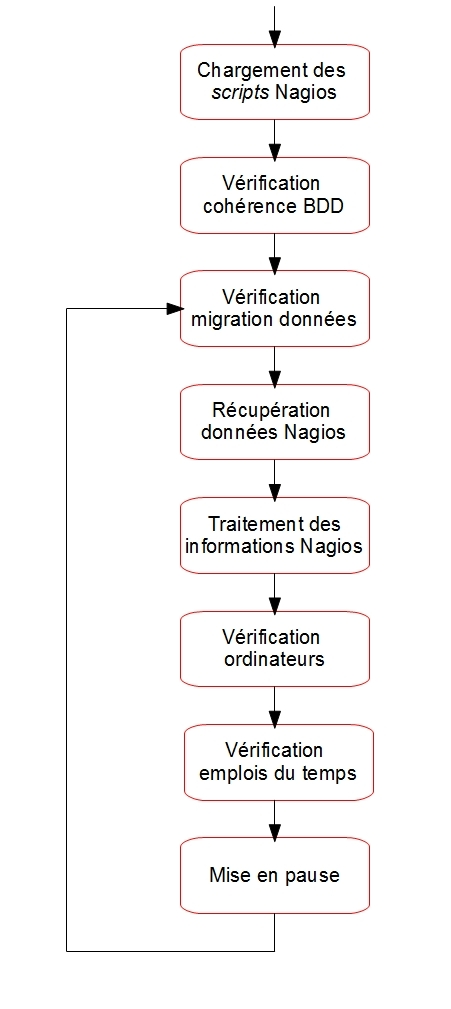
\includegraphics[scale=0.45]{cyclePrincipal.jpg}
	\caption{Sch\'ema du d\'eroulement du cycle principal du service Web}
	\label{figure:cyclePrincipal}
	
\end{figure}

Dans un premier temps, \`a la premi\`ere ex\'ecution du cycle, les diff\'erents \textit{scripts} \'ecris en LQL Nagios sont charg\'es en m\'emoire.
Ensuite, une v\'erification de la coh\'erence des donn\'ees contenues dans les tables permettant de g\'erer l'archivage des donn\'ees est effectu\'ee.
Cette v\'erification a pour but de s'assurer que il n'y a pas des donn\'ees absurdes de connexion : les donn\'ees de connexion dont dat\'ees de plus de 6 heures pour la table \textsf{yuukou\_who} et les donn\'ees de connexion dont la diff\'erence entre la date de d\'ebut de connexion et la date de fin de connexion est de plus de 6 heures elle aussi.
Si de telles donn\'ees sont trouv\'ees, elles sont automatiquement effac\'ees de la table auxquelles elles appartiennent.

L'\'etape suivante entre dans le d\'ebut du cycle \`a proprement parler.
Elle a pour objectif de v\'erifier si des donn\'ees de la table \textsf{yuukou\_last} ont besoin d'\^etre d\'eplac\'ees.
Des explications sur la migration des donn\'ees se trouvent au\S~\ref{section:migrationDonnees}.

Suite \`a cette v\'erification, les \textit{scripts} Nagios sont envoy\'es et les informations r\'ecup\'er\'ees sont transmises \`a l'\'etape de traitements des donn\'ees Nagios.

Cette \'etape commence par ajouter les machines qui n'existent pas dans la base de donn\'ees.
Ensuite, ce sont les utilisateurs qui sont trait\'es.
S'ils n'existent pas dans la base de donn\'ees, une recherche LDAP$^*$ est effectu\'ee pour obtenir les informations les concernant (nom, pr\'enom, photo, r\^ole).
Ils sont ensuite \`a leur tour, ajout\'es dans la table correspondante.
Le couple ordinateur - utilisateur est ensuite ajout\'e, mis \`a jour ou retir\'e des tables d'archivage.
Ici aussi, si une donn\'ee de connexion d\'epasse les 6 heures, elle sera ignor\'ee.

Suite \`a ce traitement, une v\'erification est effectu\'ee sur tous les ordinateurs connus.
En effet, un ordinateur poss\`ede un statut particulier : fonctionnel, \'eteint ou en attente d'effacement.
Ce statut est maintenant d'une part avec l'\'etape de traitement des r\'esultats pr\'ec\'edente, au d'autre part avec l'\'etape actuelle.
Si le statut d'un ordinateur reste \'eteint pendant une semaine, son statut change et passe \`a : en attente d'effacement.

Une v\'erification des emplois du temps est ensuite effectu\'ee.
Des explications sur la r\'ecup\'eration des emplois du temps se trouvent au \S~\ref{section:emploiDuTemps}.
Cette v\'erification a pour r\^ole de mettre \`a jour les donn\'ees sur les emplois du temps de fa\c{c}on journali\`ere.
De ce fait, tous les jours, les diff\'erents emplois du temps sont r\'ecup\'er\'es automatiquement.
\`A la suite de cette derni\`ere \'etape, le cycle se met en pause pendant une minute.

Diff\'erentes s\'ecurit\'es ont \'et\'e mises en place pour \'eviter les appels successifs au cycle principal.
En effet, quand un administrateur lance le cycle principal, il lance un processus annexe qui se charge d'effectuer le cycle ind\'efiniment.
Le seul moyen d'arr\^eter ce processus ou d'\'eviter les conflits est l'utilisation de la table \textsf{yuukou\_settings}.
Cette table permet de savoir quand un cycle a \'et\'e effectu\'e pour la derni\`ere fois et s'il est ou non en cours.
Agir sur cette table permet donc de stopper le processus mais aussi d'avoir une assurance qualit\'e sur les informations qui seront retourn\'ees par les m\'ethodes accessibles pour le client.
Si un cycle date de 5 heures, alors il ne faut pas tenir compte des informations retourn\'ees.


\subsection{Les fonctions accessibles}

\subsubsection{Les fonctions publiques}
\label{section:fonctionsPubliques}

Ces fonctions sont accessibles par tous les utilisateurs appartenant \`a l'Universit\'e.
Elles ne retournent aucunes informations pouvant porter atteinte aux utilisateurs ou pouvant donner acc\`es \`a l'administration du service Web.

\begin{description}
	\item[\textbf{healthForRoom (String idRoom)}] retourne toutes les informations concernant une salle : emploi du temps, nombre d'utilisateur, description de la salle, {\ldots} Cette fonction donne des informations d\'etaill\'ees sur une salle informatique;
	\item[\textbf{healthForAllRooms ()}] retourne des informations simplifi\'ees concernant l'ensemble des salles surveill\'ees, cette fonction donne une vue d'ensemble de l'occupation des salles;
	\item[\textbf{getListRooms ()}] retourne la liste de toutes les salles;
	\item[\textbf{getSitesInformation ()}] retourne les informations concernant les diff\'erents campus de l'Universit\'e;
	\item[\textbf{getRoomsType (String typeRoom)}] retourne la liste des salles en fonction d'un type de machine (PC ou MAC).

\end{description}

\subsubsection{Les fonctions priv\'ees}

Ces fonctions sont un compl\'ement aux fonctions publiques.
Elles permettent un contr\^ole sur le cycle principal du service Web et des informations retourn\'ees plus compl\`etes.

\begin{longdescription}
	\item[\textbf{launchCycle ()}] permet dans lancer le cycle du service Web
	\item[\textbf{checkConfigHealth ()}] compare les diff\'erences entre la table des salles informations (\textsf{yuukou\_rooms}) et la configuration dans Nagios, et retourne les diff\'erences;
	\item[\textbf{who ()}] retourne la liste de tous les utilisateurs connect\'es, sur quel ordinateur et depuis quand (\textsf{yuukou\_who});
	\item[\textbf{lastDefault ()}] retourne la table compl\`ete \textsf{yuukou\_last};
	\item[\textbf{last (int numberDays)}] retourne la table \textsf{yuukou\_last} mais pour un nombre de jours d\'efinis;
	\item[\textbf{searchHistoryUser (String idUser, boolean who, boolean last, int numberLast)}] retourne l'historique de connexion actuel (who) ou pass\'e (last) d'un utilisateur, possibilit\'e de fixer le nombre d'informations retourn\'e;
	\item[\textbf{searchHistoryResource (String idResource, boolean who, boolean last, int numberLast)}] retourne l'historique d'utilisation en cours (who) et pass\'e (last) d'un ordinateur, possibilit\'e de fixer le nombre d'informations retourn\'e;
	\item[\textbf{getGraphWithRequestUsingJson (String rqtLabel, String label, String startTime, String endTime, String addToRqt, int factor)}] retourne un flux d'octets contenant une image g\'en\'er\'ee \`a partir de la fr\'equence d'utilisation des salles informatiques entre un temps de d\'ebut et de fin (\textit{startTime} et \textit{endTime}), les donn\'ees servant \`a construire le graphe sont aussi retourn\'ees. L'\'echelle du graphe peut \^etre fix\'e avec \textit{factor} : heures, semaines, mois, ann\'ees.
Il est possible de personnalis\'er la requ\^ete (\textit{addToRqt}), de personnaliser la l\'egende (\textit{label}) et de choisir l'\'el\'ement recherch\'e (\textit{rqtLabel});
	\item[\textbf{healthResourcesReportForAllRooms ()}] retourne l\'etat des ordinateurs de toutes les salles informatiques surveill\'ees;
	\item[\textbf{healthResourcesReportForRoom (String idRoom)}] retourne l'\'etat des ordinateurs d'une salle sp\'ecifique;
	\item[\textbf{actualiseLDAPInfo ()}] permet d'actualiser les donn\'ees LDAP des utilisateurs qui sont inconnus dans la base de donn\'ees;
	\item[\textbf{isCycleRunning ()}] donne l'\'etat du cycle, s'il est en cours ou non;
	\item[\textbf{askMaintenance ()}] si le cycle n'est pas en cours, modifie la table de configuration pour stopper le cycle \`a sa prochaine it\'eration.
Tout lancement de cycle est impossible ensuite;
	\item[\textbf{endMaintenance ()}] met fin \`a la maintenance, le cycle peut ensuite \^etre relanc\'e;
	\item[\textbf{isMaintenanceScheduled ()}] permet de savoir si une maintenance est en cours ou non.

\end{longdescription}

\subsection{Retours des fonctions}
\label{section:retourFonction}

\'Etant dans un cadre de travail collaboratif comme le traitera le \S~\ref{section:travailequipe}, il est n\'ecessaire d'adopter de la rigueur dans le retour d'information.
Encore plus du fait qu'en JSON, le fichier ne peut pas \^etre v\'erifi\'e comme un fichier XML et son sch\'ema.
C'est pourquoi, deux mani\'eres sp\'ecifiques ont \'et\'e choisies pour retourner les informations : le cas o\`u les informations on \'et\'e correctement transmises et le cas o\`u elles ne l'ont pas \'et\'e.
Des exemples de retours concrets sont disponibles en annexe~\ref{chapterAnnexe:exempleJSON}.

\subsubsection{Retour de fonction pour une ex\'ecution correcte}

La structure d'un retour d'une fonction suit toujours le m\^eme sch\'ema.
Le bout de code JSON~\ref{figure:structureSansErreurJSON} montre un exemple de structure de retour lorsqu'aucune erreur n'est d\'etect\'ee pendant l'ex\'ecution d'une m\'ethode du service Web.

\begin{figure}[!ht]
	\centering
	\lstinputlisting[language=JSON]{codes/structureSansErreur.json}
	\caption{Structure g\'en\'erale de retour de fonction JSON sans erreur}
	\label{figure:structureSansErreurJSON}

\end{figure}

\subsubsection{Retour de fonction pour une ex\'ecution incorrecte}

Le bout de code JSON~\ref{figure:structureAvecErreurJSON} montre un exemple de structure de retour lorsqu'une erreur est d\'etect\'ees pendant l'ex\'ecution d'une m\'ethode du service Web.

\begin{figure}[!ht]
	\centering
	\lstinputlisting[language=JSON]{codes/structureAvecErreur.json}
	\caption{Structure g\'en\'erale de retour de fonction JSON avec erreur}
	\label{figure:structureAvecErreurJSON}

\end{figure}


%%%%%%%%%%%%%%%%%%%%%%%%%%%
% FONCTIONNALITES WS %%%%%%
%%%%%%%%%%%%%%%%%%%%%%%%%%%
\section{Fonctionnalit\'es en place}

\subsection{Gestion de la base de donn\'ees}

La base de donn\'ees a \'evolu\'e tout au long du projet en fonction des fonctionnalit\'es qui ont \'et\'e demand\'ees.
L'annexe~\ref{chapterAnnexe:baseDeDonnees} permet d'avoir une description des diff\'erentes tables composant la base de donn\'ees, une vue g\'en\'erale de ce \`a quoi elle ressemble, et des vues d\'ecoup\'ees des diff\'erentes parties.

La base de donn\'ees peut \^etre d\'ecoup\'ee en diff\'erentes grandes parties.
La partie archivage a pour but de conserver les donn\'ees dans le temps.
Pour ce faire, elle est compos\'ee de deux tables centrales de sauvegarde d'informations.
La premi\`ere est la table \textsf{yuukou\_who}, son but est de simuler la commande UNIX \textsf{who}.
Cette commande permet de donner tous les utilisateur connect\'es sur la machine o\`u elle est ex\'ecut\'ee.
De ce fait, si elle est port\'ee au niveau de Nagios et du projet, la table contiendra tous les utilisateurs connect\'es sur un ordinateur et depuis quand ils le sont.
La deuxi\`eme table est \textsf{yuukou\_last}, son but est aussi de simuler une commande UNIX, la commande \textsf{last}.
Cette commande permet de donner la liste de toutes les derniers utilisateurs sur la machine sur laquelle elle est ex\'ecut\'ee.
De ce fait, si elle est port\'ee au niveau de Nagios et du projet, la table contiendra toutes les connexions des utilisateurs sur un ordinateur, l'heure de d\'ebut et de fin et la cause de la d\'econnexion. En fait, elle contiendra les donn\'ees de la table \textsf{yuukou\_who} et ajoutant les informations du temps de fin de connexion et la cause de la d\'econnexion.

La partie logicielle a pour but de stocker la configuration logicielle de chaque salle informatique.
La r\'ecup\'eration de cette configuration est expliqu\'ee au \S~\ref{section:catalogueLogiciel}.
Cette partie est compos\'ee de plusieurs tables.
Une salle informatique peut avoir des groupes de logiciels, \textsf{yuukou\_rooms\_groups} et aussi des logiciels ind\'ependants de tout groupe, \textsf{yuukou\_rooms\_software}.
Un groupe de logiciels contient des logiciels, \textsf{yuukou\_groups\_software}.
Les descriptions des groupes et logiciels sont contenues dans les tables \textsf{yuukou\_groups} et \textsf{yuukou\_software}.
Avec ces tables, il est possible de facilement reconstruire la configuration logicielle d'une salle.

La partie emploi du temps a pour but de stocker tous \'ev\`enements des diff\'erents emplois du temps de l'Universit\'e.
La r\'ecup\'eration de cette configuration est expliqu\'ee au \S~\ref{section:emploiDuTemps}.
Cette partie est compos\'ees de trois tables.
La premi\`ere table est celle contenant toutes les salles \textsf{yuukou\_rooms}, la deuxi\`eme contenant tous les \'ev\`enements \textsf{yuukou\_timetables}.
Pour la derni\`ere table \textsf{yuukou\_mapping\_room}, son r\^ole est de faire le lien entre les noms des salles dans Nagios et les noms des salles qui sont utilis\'ees pour l'emploi du temps.
En effet, la g\'en\'eration des emplois du temps est effectu\'ee par un service de l'Universit\'e.
De ce fait, ce service utilise un syst\`eme pour nommer les salles qui lui est propre.
Il est donc n\'ecessaire de pouvoir relier un \'ev\`enement \`a une salle \`a l'aide de cette derni\`ere table.

La partie \textit{mapping} avec les salles a pour but de faire le lien entre une description compl\`ete d'un lieu et la description courte qui est donn\'e dans la description d'une salle dans la table \textsf{yuukou\_rooms}.
Les informations concernant les diff\'erents lieux sont contenues dans la table \textit{yuukou\_mapping\_location}.

La derni\`ere partie, configuration, a pour but de g\'erer les diff\'erents param\`etres permettant la gestion de cycle lors du fonctionnement du service Web. 
Les explications concernant ce qu'est un cycle se trouvent au \S~\ref{section:cyclePrincipal}.

\subsection{S\'ecurisation du service Web}
\label{section:securisation}

\subsubsection{Explications}

La s\'ecurit\'e est un point important dans l'acc\`es \`a un service Web. 
Les donn\'ees transmises par \YuukouII{} contiennent des informations sur la structure des diff\'erents campus mais aussi des informations sur les \'etudiants (nom, pr\'enom, photo par exemple).
Il est donc important de limiter l'acc\'es aux donn\'ees mais aussi de s\'ecuriser toutes les communications.
C'est dans cet optique, qu'il a \'et\'e d\'ecid\'e de mettre en place le protocole SSL entre le service Web et toute application voulant communiquer avec.

Le protocole \textit{Secure Sockets Layer}, ou SSL, est con\c{c}u pour assurer la confidentialit\'e, l'authentification et l'int\'egrit\'es des donn\'ees lorsdes \'echanges entre un client et un serveur Web, sur diff\'erents protocoles de transport (en g\'en\'eral HTTP).
SSL met en place un chiffrement \`a cl'es publiques, \cad, une combinaise de deux cl\'es : une cl\'e publique servant au chiffrement des donn\'ees et une cl\'e priv\'ee servant au d\'echiffrement.
Les sites Internet b\'en\'eficiant de ce protocole sont reconnaissables du fait de leurs URL\protect\footnote{\textit{Uniform Resource Locator}} commen\c{c}ant par \textsf{https://} o\`u le 's' signifie \textit{secured}.

\subsubsection{Fonctionnement}

\noindent La mise en place d'un tunnel SSL entre client et serveur se fait en 4 \'etapes :

\begin{enumerate}
	\item le client fait une demande de connexion s\'ecuris\'ee, il demande donc le certificat garantissant la cl\'e publique du serveur;
	\item le serveur lui envoie son certificat d'authentification d\'elivr\'e par l'autorit\'e de certification, ce certificat contient la cl\'e publique;
	\item si l'autorit\'e de certification et le certificat sont valide, alors le client envoie une cl\'e secr\`ete, cr\'e\'ee \`a partir de la cl\'e publique;
	\item le client et le serveur poss\`ede maintenant une cl\'e secr\`ete qui sera encrypt\'e \`a l'aide d'un algorithme de hachage pour plus de s\'ecurit\'e.
	Si la connexion est perdue, une nouvelle cl\'e secr\`ete sera n\'egoci\'ee.

\end{enumerate}

\subsubsection{Mise en place}

La mise en place d'un protocole SSL sur un service Web via NetBeans et GlassFish est tr\`es simple.
Il faut cependant disposer de plusieurs fichiers : une autorit\'e de certification et un couple cl\'e priv\'e - cl\'e publique tous deux fournis par l'Universit\'e.
\`A partir de ces deux fichiers, un certificat de s\'ecurit\'e est g\'en\'er\'e.
Ensuite l'autorit\'e de certification et le nouveau certificat sont ajout\'es \`a la configuration de GlassFish.

La configuration avec NetBeans consiste \`a pr\'eciser que le service Web utilisera une connexion s\'ecuris\'ee de type SSL sur toutes les m\'ethodes HTTP (Get, Post, \ldots).
Apr\`es d\'eploiement, le service Web ne sera accessible qu'avec HTTPS et le certificat sera diffus\'e.


\subsection{G\'en\'eration de graphes d'utilisation}

Afin de rajouter des fonctionnalit\'es au service Web, il a \'et\'e mis en place une m\'ethode permettant de g\'en\'erer des graphes d'utilisation sous forme d'une image.
Basiquement, une requ\^ete est ex\'ecut\'ee sur la table \textsf{yuukou\_last}, les donn\'ees sont compt\'ees et la g\'en\'eration d'un graphe est effectu\'ee.

La g\'en\'eration de graphes utilise l'API$^*$ RRD4J.
Cette API$^*$ est en fait l'impl\'ementation Java de RRDtool.
RRDtool est un outil de gestion de base de donn\'ees RRD (\textit{Round-Robin Database}).
C'est un outil \textit{open source} permettant le stockage et la g\'en\'eration de graphes \`a partir de donn\'ees chronologiques.
RRDtool est utilis\'e avec notamment Nagios et Cacti par exemple.

Dans le cadre du projet, l'utilisation r\'eelle de ce logiciel a \'et\'e d\'etourn\'ee du fait que normalement, les donn\'ees sont constamment archiv\'ees.
En fait, \`a chaque demande de graphes, une nouvelle table RRD est cr\'e\'ee, remplie, exploit\'ee pour obtenir une image de graphe puis effac\'ee.
Le but n'\'etait pas une int\'egration parfaite au service Web, mais un aper\c{c}u des possibilit\'es qu'offre RRDtool.

La figure~\ref{figure:rrdTool} pr\'esente un exemple de graphe d'utilisation des salles informatiques de l'Universit\'e \`a l'aide de l'API$^*$ RRD4J pendant une journ\'ee.

\begin{figure}[!ht]
	\centering
	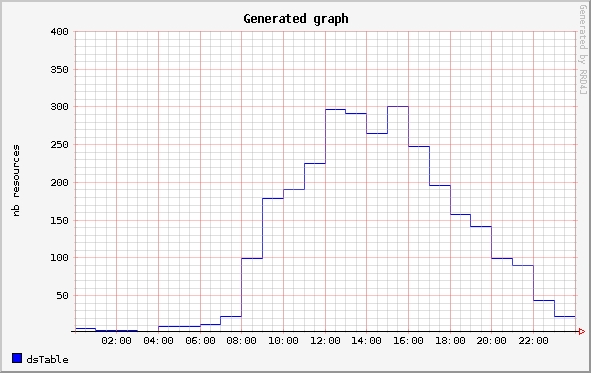
\includegraphics[scale=0.5]{exempleRRDtool.jpg}
	\caption{Exemple de graphe d'utilisation des salles informatiques de l'Universit\'e g\'en\'er\'e avec RRD4J}
	\label{figure:rrdTool}

\end{figure}

\subsection{Gestion de l'emploi du temps}
\label{section:emploiDuTemps}

\subsubsection{Les flux RSS de l'Universit\'e}

Pouvoir donner l'\'etat d'une salle informatique a un \'etudiant est un point cl\'e du service Web.
En effet, donner l'occupation d'une salle sans prendre en compte le fait qu'un cours puisse s'y d\'erouler n'est pas suffisant.
Il est ainsi n\'ecessaire de savoir l'occupation d'une salle : le nombre d'ordinateurs libre, mais aussi si l'emploi du temps de cette salle permet de venir y travailler.

L'Universit\'e met \`a disposition 4 flux RSS$^*$ contenant toutes les informations sur l'occupation des salles.
Ces 4 flux correspondent aux 4 grands campus de l'Universit\'e : Harrow, New Canvendish, Marylebone et Regent.
Ils pr\'esentent l'avantage d'\^etre \'ecris en XML, de ce fait, le contenu des flux peut \^etre r\'ecup\'er\'e.
Les informations permettant d'identifier un \'ev\`enement sont extraites \`a l'aide d'un \textit{parseur} de type DOM$^*$.
Chaque \'ev\`enement est ensuite ajout\'e dans la base de donn\'ees.

\subsubsection{Correspondance des salles}

Les noms des salles informatiques contenus dans les flux RSS$^*$ et ceux pr\'esents dans {\YuukouII} ne sont pas les m\^emes.
Cela vient du fait que les flux existent depuis longtemps, de ce fait, les \'equipes charg\'ees de leurs maintenance ont adopt\'es leur propre syst\`eme de nommage des salles.
Un table interm\'ediaire a donc \'et\'e cr\'e\'ee pour faire la relation entre une salle de {\YuukouII} et une salle de l'emploi du temps.
Cependant, le nommage ambigu des salles dans les diff\'erents flux d'emploi du temps fait que seules quelques salles ont une correspondance dans le projet.
Une discussion a eu lieu \`a ce sujet dans le but d'adopter un syst\`eme logique permettant de faire une correspondance plus facile avec toutes les salles surveill\'ees.
Mais la mise en place d'un tel syst\`eme n'est pas pr\'evu dans l'imm\'ediat.

\subsection{Catalogue logiciels des salles}
\label{section:catalogueLogiciel}

Un des objectifs final de {\YuukouII} est de fournir \`a \'etudiant une liste des logiciels pouvant \^etre utilis\'es dans chaque salle.
Le but \'etant, qu'un \'etudiant, voulant travailler dans une salle libre sur un logiciel sp\'ecifique comme Visual Studio, puisse trouver rapidement les salles qui correspondent \`a ses attentes.

Il existe un \textit{MediaWiki} mettant \`a disposition des membres de l'Universit\'e, des informations sur les salles telles que : une photo de la salle, une description, les responsables et la configuration logicielle de la salle.
Un \textit{MediaWiki} est un logiciel permettant de r\'ealiser des sites Internet de type wiki$^*$. 
Il s'agit d'un syst\`eme de gestion de contenu de sites Web qui rend les pages Web librement modifiables par tous les visiteurs autoris\'es.
Le site Web \textit{Wikip\'edia} (\url{http://fr.wikipedia.org/wiki/Wikip\%C3\%A9dia:Accueil\_principal}) a \'et\'e d\'evelopp\'e avec \textit{MediaWiki}.

Afin de faciliter la gestion de sites Web de ce genre, de nombreuses API$^*$ existent.
C'est donc en utilisant une de ces API$^*$ que la configuration logicielle de chaque salle a \'et\'e r\'ecup\'er\'ee.
Les diff\'erents logiciels et groupes de logiciels sont extraits et les diff\'erents liens sont contruits puis ajout\'es \`a la base de donn\'ees.
Cependant, il est \`a noter que le \textit{MediaWiki} ne concerne que quelques salles de la \textit{School of Electronics and Computer Science}.

\subsection{Migration des donn\'ees}
\label{section:migrationDonnees}

Pendant le d\'eveloppement du projet, vue la quantit\'e de donn\'ees contenues dans la table \textsf{yuukou\_last} (environ 50 000 \`a 60 000 entr\'ees par mois), la question de l'archivage de ses donn\'ees s'est pos\'ee.
Une m\'ethode a donc \'et\'e recherch\'ee en consid\'erant le fait que les donn\'ees archiv\'ees peuvent \^etre r\'eutilis\'ees lors de l'ex\'ecution de quelques m\'ethodes par le client.

Une solution a \'et\'e trouv\'ee : le d\'eplacement \`a chaque d\'ebut de mois des donn\'ees dans une nouvelle table.
Chaque nouvelle table est identifi\'ee de la sorte : 

\begin{center}
	\textsf{yuukou\_last \_ ann\'ee mois}

\end{center}

Avec un exemple pour illustrer, \'etant en juin 2012, la table archiv\'ee correspondant au mois de mai portera le nom suivant : 

\begin{center}
	\textsf{yuukou\_last\_201205}

\end{center}

De cette mani\`ere, les donn\'ees contenues dans la table \textsf{yuukou\_last} correspondent aux mois en cours.


%%%%%%%%%%%%%%%%%%%%%%%%%%%
% ORGANISATION TRAVAIL %%%%
%%%%%%%%%%%%%%%%%%%%%%%%%%%
\section{Organisation du travail}

Une rigueur dans le d\'eroulement d'un projet permet d'\'eviter de nombreuses difficult\'es.
C'est d'autant plus le cas quand le projet comprend plusieurs personne comme c'est le cas pour {\YuukouII}.
De ce fait, cette partie permet de comprendre comment s'organisait le travail au sein de l'Universit\'e.
Dans un premier temps sera abord\'ee la gestion du poste de travail, \cad, la strat\'egie de d\'eveloppement.
Ensuite, le d\'eroulement du travail en \'equipe sera expliqu\'e, le projet \'etant un travail collaboratif entre une partie service Web et une partie affichage.
Et dans la derni\`ere partie sera vue la fa\c{c}on de tester le service Web avant de le consid\'erer comme stable.

\subsection{Gestion du poste de travail}
\label{section:gestionProjet}

Afin de d\'evelopper efficacement, une organisation du poste de travail mais plus g\'en\'eralement du projet en lui-m\^eme a \'et\'e choisie.
Cette organisation comporte une machine de d\'eveloppement et deux serveurs comme le montre la figure~\ref{figure:gestionProjet}.

\begin{figure}[!ht]
	\centering
	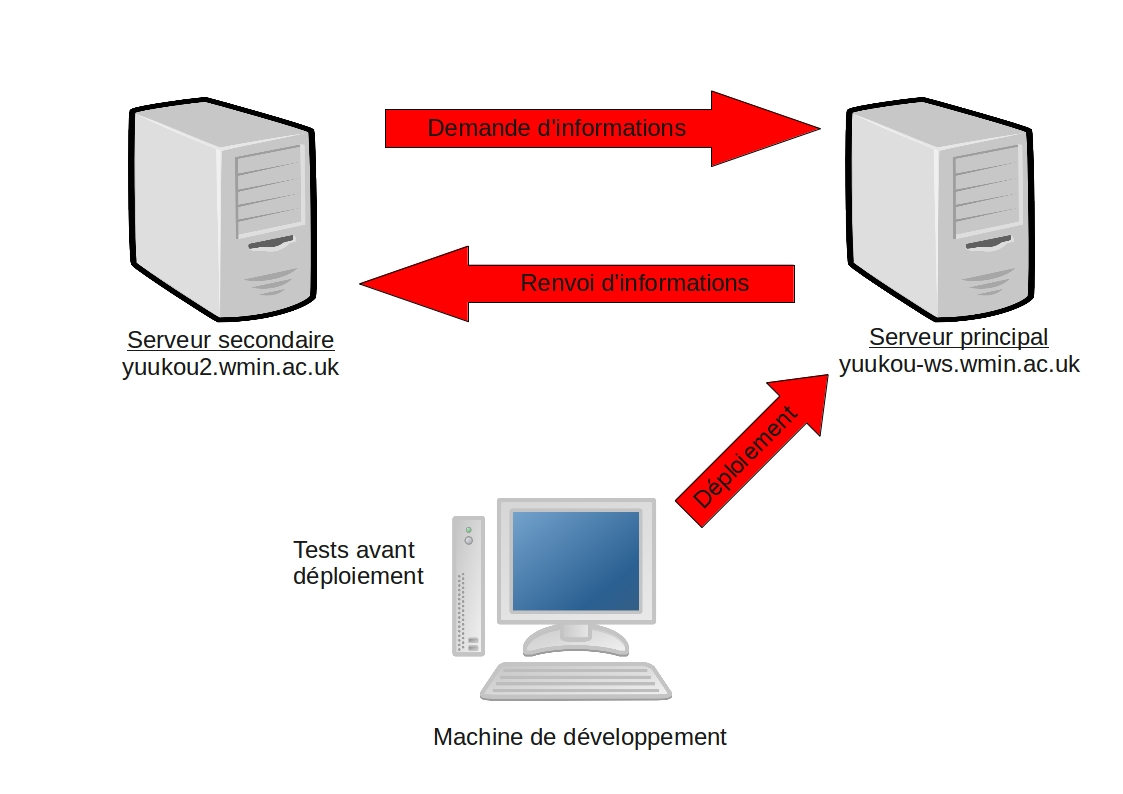
\includegraphics[scale=0.34]{gestionProjet.jpg}
	\caption{Sch\'ema de la gestion du projet}
	\label{figure:gestionProjet}

\end{figure}

Le serveur principal poss\`ede un syst\`eme d'exploitation Debian version 6.0.5 (\textit{Squeeze}) et h\'eberge le service Web dans une version stable ainsi que tous les outils n\'ecessaire \`a son fonctionnement comme le serveur de gestion de base de donn\'ees (SGBD) MySQL, une version de Java \`a jour, le serveur d'application GlassFish mais aussi Nagios.
La faible consommation CPU de Nagios dans la surveillance des machines de l'Universit\'e fait, qu'actuellement, il peut \^etre h\'eberg\'e sur le m\^eme serveur que le service Web.
Le serveur principal h\'eberge aussi le gestionnaire de version subversion (SVN) sur lequel est constamment maintenu le projet.
Il est accessible sur le r\'eseau sous le nom de domaine \textsf{yuukou-ws.wmin.ac.uk}.

Le serveur dit {\og}secondaire{\fg} poss\`ede lui aussi le m\^eme syst\`eme d'exploitation Debian et h\'eberge l'application Web permettant de communiquer avec le service Web.
Cette application fait r\'eguli\`erement appel au service Web pour obtenir les informations dont elle a besoin pour afficher correctement ses pages.
Il est accessible sur le r\'eseau sous le nom de domaine \textsf{yuukou2.wmin.ac.uk}.

La machine de d\'eveloppement poss\`ede un syst\`eme d'exploitation Linux Mint version 11 (\textit{Katya}), tous les outils n\'ecessaires au d\'eveloppement (comme Java, NetBeans, \ldots), mais aussi un serveur de gestion de base de donn\'ee (SGBD) MySQL et un serveur GlassFish, tous deux servant \`a effectuer des tests avant d\'eploiement.
\`A chaque d\'eploiement sur le serveur principal, la version du projet est publi\'ee sur le SVN afin de garantir une s\'ecurit\'e dans le cas d'une r\'egression dans le d\'eveloppement.

\subsection{Travail en \'equipe}
\label{section:travailequipe}

Le projet {\YuukouII}, comme \'enonc\'e dans le \S~\ref{section:architectureProjet}, a \'et\'e divis\'e en deux parties.
La partie service Web, permettant de remplir et maintenir la base de donn\'ees ainsi que de mettre \`a disposition d'un client des m\'ethodes retournant une partie des informations r\'ecup\'er\'ees, et la partie affichage dont le r\^ole est de pr\'esenter les informations \`a un utilisateur lambda.
La partie affichage fut confi\'ee \`a Yacine MAGHEZZI, \'etudiant en 3\up{i\`eme} ann\'ee de Licence informatique \`a l'Universit\'e de Franche-Comt\'e de Besan\c{c}on, ainsi qu'\`a M. Thierry DELAITRE et Anne-Gaelle COLOM, venus apporter leurs contributions par la suite.
Le but de ce projet \'etait, \`a l'aide du service Web, de permettre un affichage r\'esumant la disponibilit\'e des laboratoires informatiques dans l'Universit\'e.

Ainsi, \`a chaque red\'eploiement du service Web lors d'une mise \`a jour importante ou d'un ajout de fonctionnalit\'es, il \'etait important de les tenir inform\'e des diff\'erents changements qui ont \'et\'e effectu\'es.
C'est dans le cadre de ce travail en \'equipe que des structures de retour standard a \'et\'e adopt\'ee (voir \S~\ref{section:retourFonction}).
En effet, un minimum de rigueur dans le d\'eveloppement permettait de ne pas avoir de surprises \`a chaque \'etape du projet.

Cependant, la majeure partie de la communication se faisait selon les besoins des diff\'erents d\'eveloppeurs.
Avant l'arriv\'ee de M. MAGHEZZI, les fonctionnalit\'es et les informations qu'elles retournaient n'\`etaient que limit\'ees.
Cela \'etant d\^u au fait que elles n'\'etaient exploit\'ees par personne.
Apr\`es son arriv\'ee et sa premi\`ere connexion au service Web, M. MAGHEZZI a commenc\'e \`a exprimer des demandes concernant les \'el\'ements qu'il aimerait voir appara\^itre.
C'est \`a ce moment que le dialogue s'est vraiment mis en place.

\'Etant dans le m\^eme bureau que M. MAGHEZZI, la communication se d\'eroulait principalement oralement, il \'etait inform\'e directement et m\^eme en avance par rapport au d\'eploiement d'une nouvelle version du service Web.
Pour les autres acteurs du projet, un mail \'etait envoy\'e, celui-ci contenant tr\`es souvent des structures de retour JSON contenant le sch\'ema d'une structure de retour de tous les cas possibles pour une m\'ethode sp\'ecifique du service Web.

\subsection{Tests du service Web}

Le d\'eploiement du service Web sur le serveur principal impose d'avoir une version stable et sans bogue.
De ce fait, comme expliqu\'e au \S~\ref{section:gestionProjet}, le service Web est une premi\`ere fois d\'eploy\'e sur la machine de d\'eveloppement.
Afin de v\'erifier son bon fonctionnement, un service Web client a \'et\'e mis en place.
Ce client ouvre une connexion s\'ecuris\'ee, puis donne acc\`es aux m\'ethodes qu'il est possible de tester sur le service Web.
Il agit comme l'application permettant l'affichage des donn\'ees du service Web que M. MAGHEZZI a cr\'e\'e, \`a la diff\'erence que les r\'esultats sont affich\'es en texte brut.

Le client donc d\'evelopp\'e en tant que service Web client.
Les pages Web sont g\'en\'er\'ees gr\^ace \`a des \textit{Servlet}$^*$ Java.
Il est a not\'e la pr\'esence d'un \textit{Servlet} permettant la gestion du cycle principal.
Il offre donc un contr\^ole sur le cycle : d\'emarrage, mise en maintenance et fin de la maintenance.


%%%%%%%%%%%%%%%%%%%%%%%%%%%
% EXPLOITATION WS %%%%%%%%%
%%%%%%%%%%%%%%%%%%%%%%%%%%%
\section{Exploitation du service Web}

Le service Web est directement interrog\'e par la partie affichage du projet.
Cette partie affichage se pr\'esente sous la forme d'une interface homme-machine (IHM) d\'evelopp\'ee gr\^ace aux technologies JSP, Servlet et jQuery Mobile.
Cette application pr\'esente, en fonction de diff\'erents niveaux de s\'ecurit\'e, diff\'erentes vues.

Un utilisateur normal, comme un \'etudiant, aura une vue sur la disponibilit\'e des salles informatiques.
Il pourra voir toutes les salles, leur disponibilit\'es (ordinateurs disponibles, occup\'es, \'eteints, salle disponible ou occup\'ee par un \'ev\`enement de l'emploi du temps), les filtrer par lieu, ou encore par type d'ordinateur (PC ou MAC).

Un membre des \'equipes techniques de l'Universit\'e (staff) aura une vue la disponibilit\'e des salles informatiques en plus d'une vue sur le mat\'eriel.
Il aura acc\`es \`a des graphiques, des r\'esum\'es de l'occupation des salles mais aussi \`a des informations suppl\'ementaires sur les salles (informations sur les utilisateurs connect\'es et historique des ordinateurs).

La figure~\ref{figure:exempleIPhone} donne trois vues diff\'erentes sur ce que l'application d'affichage des donn\'ees du service Web propose.
Les figures sont des captures d\'ecrans prises \`a l'aide d'un \'emulateur d'IPhone.
Il est a not\'e que les figures suivantes ont \'et\'e prises en s'authentifiant avec un compte utilisateur.
Comme pr\'ec\'edemment annonc\'e, les staffs b\'en\'eficieront, dans certaines pages, de plus d'options.

\begin{figure}[!ht]
	\centering
	\subfloat[Listes des salles]{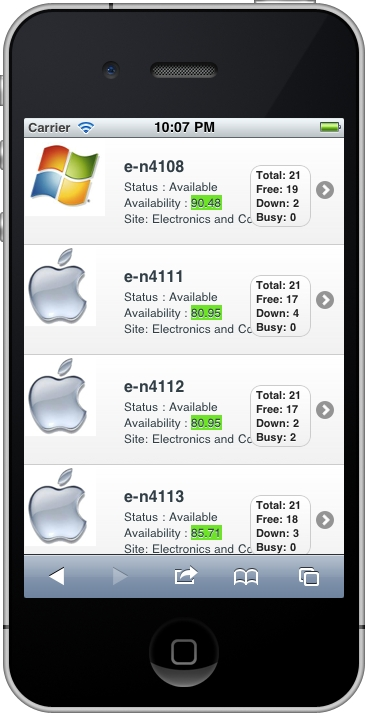
\includegraphics[scale=0.30]{phone.jpg}\label{figure:exempleIPhone:fig1}}
	\qquad
	\subfloat[Description d'une salle]{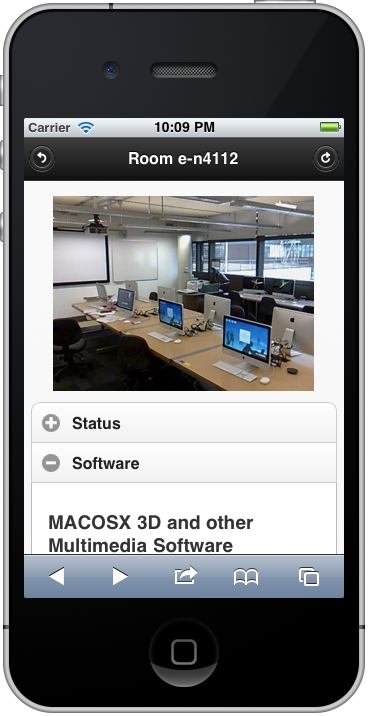
\includegraphics[scale=0.30]{phone1.jpg}\label{figure:exempleIPhone:fig2}}
	\qquad
	\subfloat[Salles occup\'ees]{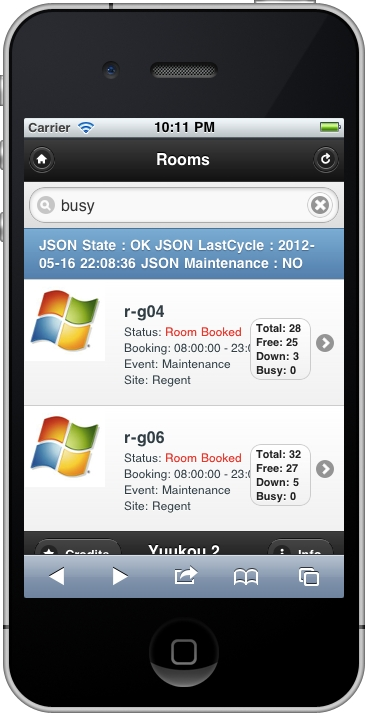
\includegraphics[scale=0.30]{phone2.jpg}\label{figure:exempleIPhone:fig3}}
	\caption{Exemples de captures d'\'ecran sur un IPhone de l'application affichant les informations du service Web}
	\label{figure:exempleIPhone}

\end{figure}

La figure~\subref{figure:exempleIPhone:fig1} montre une vue g\'en\'eraliste de la liste des salles informatiques dans l'Universit\'e.
Sur la gauche, le statut et le lieu de chaque salle sont affich\'es. 
Le statut permet de savoir si un cours se d\'eroule dans la salle ou non comme le montre la figure~\subref{figure:exempleIPhone:fig3}.
Des couleurs permettent de se rendre rapidement compte de la disponibilit\'e des salles.
Information suppl\'ementaire en l'image qui est affich\'ee : le symbole de Windows est pr\'esent afin de sp\'ecifier que la salle est une salle contenant des PC, le symbole de Macintosh est pr\'esent pour les salles contenant exclusivement des MAC.
Un r\'ecapitulatif sur la droite permet de voir le nombre total d'ordinateurs, ceux qui sont occup\'es, libres ou \'eteints.

En s\'electionnant une salle, une page contenant la description de cette salle s'affiche comme le montre la figure~\subref{figure:exempleIPhone:fig2}.
Cette description contient l'image de la salle, un commentaire sur la salle, le r\'ecapitulatif du statut et de la disponibilit\'e de la salle comme pour la figure~\subref{figure:exempleIPhone:fig1}, la configuration logicielle de la salle, un lien vers Google Map pour situer l'emplacement dans Londres et des informations compl\'ementaires (responsables de la salle, adresse compl\`ete, \ldots).

La figure~\subref{figure:exempleIPhone:fig3} montre une vue avec une recherche des salles occup\'ees dans l'Universit\'e.
Des informations apparaissent sur l'\'ev\`enement qui se d\'eroule actuellement dans les salles et la p\'eriode d'occupation des salles.
Sont toujours disponibles le type d'ordinateurs dans la salle et leur disponibilit\'e.



%%%%%%%%%%%%%%%%%%%%%%%%%%%
% PROBLEMES RENCONTRES %%%%
%%%%%%%%%%%%%%%%%%%%%%%%%%%
\section{Probl\`emes rencontr\'es}

Durant toute la dur\'ee du projet, de nombreux probl\`emes ont \'et\'e rencontr\'es.
Ils \'etaient principalement dus au manque de connaissances dans le domaine vis\'e.

Le SSL\protect\footnote{\textit{Secure Sockets Layer}} a \'et\'e difficilement mis en place dans les premiers temps.
En effet, le manque de connaissance dans les services Web et dans les outils NetBeans et GlassFish ont \'et\'e un frein dans sa mise en place.
De plus, la documentation sur le Web est plus ou moins \'evasive et les m\'ethodes sont diverses pour s\'ecuriser un service Web.
Cependant, avec l'aide de l'Universit\'e, notamment en fournissant les diff\'erents certificats et les instructions, le protocole a pu \^etre mis en fonction.

Il est apparu pendant le stage que les diff\'erents services de l'Universit\'e n'appliquaient que rarement les m\^emes normes.
Cela s'est fait ressentir dans la mise en place de la gestion des emplois du temps.
Effectivement, les noms des salles entre {\YuukouII} et ceux dans les emplois du temps n'avaient rien \`a voir.
Certes, certaines pouvaient \^etre devin\'ees, elles ont \'et\'e de ce fait trait\'ees.
Mais pour d'autres cela s'av\'erait impossible, surtout si on consid\`ere que plusieurs personnes s'occupent des emplois du temps et que ces personnes appliquent chacun une m\'ethode de nommage plus ou moins diff\'erentes les unes des autres.
Une r\'eunion a eu lieu pendant le stage avec l\'equipe en charge afin d'aborder ce point.
Au final, un nouveau syst\`eme d'identification des salles devrait \^etre mis en place, mais le service \'etant occup\'e, il n'y a pas de date dans la mise en fonction d'une telle mesure.
Lorsque ce syst\`eme sera appliqu\'e, la liste des nouveaux noms de salles sera communiqu\'ee, ce qui rendra cette partie pleinement fonctionnelle.

%TODO a finir



\clearpage


\chapter{Bilan}

\section{Bilan du travail r\'ealis\'e}

Ce bilan r\'esumera le travail r\'ealis\'e durant le stage.
Dans une premi\`ere partie, un r\'ecapitulatif du projet sera donn\'e, avec notamment un graphique afin de montrer les fonctionnalit\'es reprises de {\Yuukou} ainsi que les diff\'erentes fonctionnalit\'es qu'apporte {\YuukouII}.
Ensuite le calendrier des 16 semaines de stage, avec les diff\'erentes t\^aches effectu\'ees semaines apr\`es semaines.
Il sera suivi par une partie donnant ce qu'apporte le projet \`a l'Universit\'e, les avantages qu'elle peut en tirer.
Enfin une derni\`ere partie traitera des am\'eliorations qu'il est possible d'apporter au service Web afin d'accro\^itre ses performances et ses fonctionnalit\'es.

\subsection{R\'ecapitulatif du projet}

La figure~\ref{figure:yuukouEtYuukouII} permet de donner une vue d'ensemble sur les principales fonctionnalit\'es dont le projet dispose.
Les cadres pleins repr\'esentent des fonctionnalit\'es dont le principe a \'et\'e repris de {\Yuukou}, les cadres en pointill\'es, quant \`a eux, repr\'esentent les nouvelles fonctionnalit\'es qu'apporte \YuukouII.

\clearpage

\begin{figure}[!ht]
	\centering
	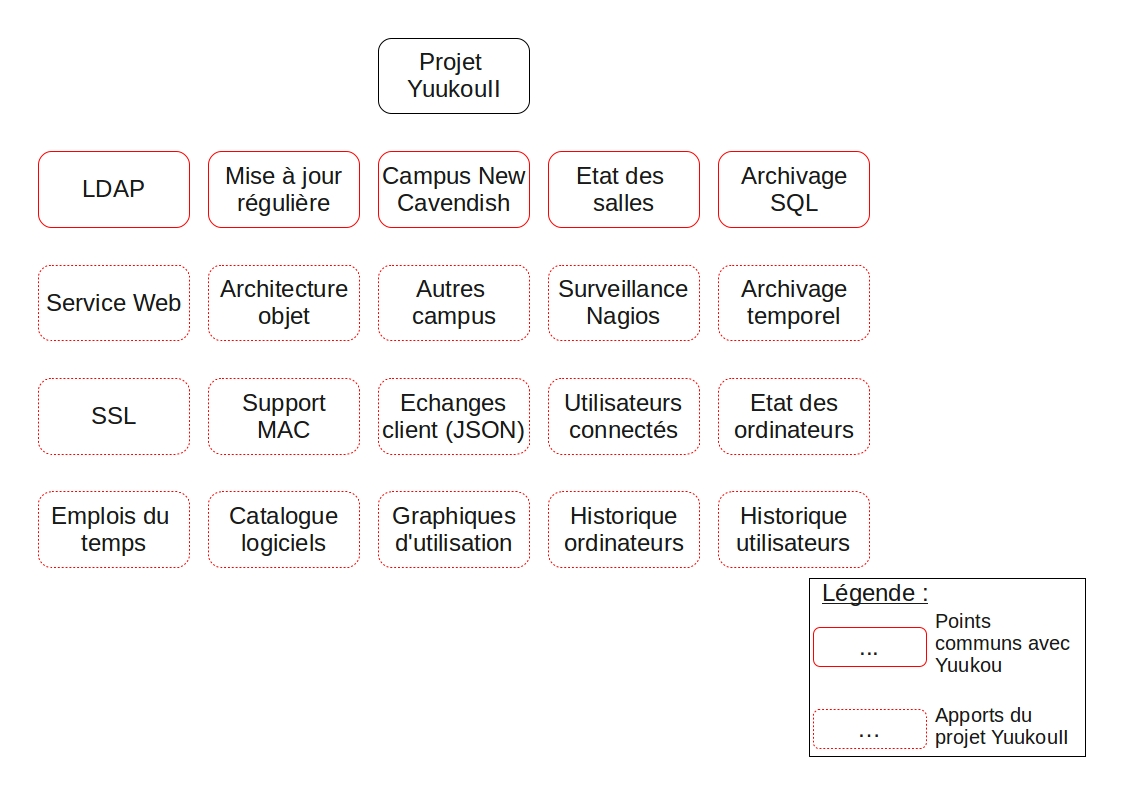
\includegraphics[scale=0.375]{yuukouEtYuukouII.jpg}
	\caption{R\'ecapitulatif des fonctionnalit\'es reprises de {\Yuukou} et les nouvelles de \YuukouII}
	\label{figure:yuukouEtYuukouII}

\end{figure}

\subsection{Calendrier du stage}

Voici le calendrier du stage d'une dur\'ee de 16 semaines commen\c{c}ant le 13 f\'evrier 2012 et terminant le 4 juin 2012.
Certains points ont demand\'e plus de travail que d'autres, comme la conception du cycle principal du service Web ou encore la mise en place du SSL qui a pos\'ee quelques difficult\'es.

\begin{description}
	\item[semaine 1] : Arriv\'ee et d\'ecouverte du projet, premier entretien avec l'\'equipe technique et leurs attentes;
	\item[semaine 2] : D\'ecouverte des services Web et choix des outils utilis\'es;
	\item[semaine 3 et 4] : Conception de la base de donn\'ees et impl\'ementation du cycle principal de l'application;
	\item[semaine 5] : Mise en place de l'emploi du temps et d\'ebut mise en place de SSL;
	\item[semaine 6] : Mise en place du syst\`eme JSON et fin de mise en place de SSL;
	\item[semaine 7 et 8] : D\'eveloppement des m\'ethodes Web;
	\item[semaine 9] : Mise en place de l'architecture finale et d\'eveloppement des m\'ethodes Web;
	\item[semaine 10] : D\'ebut de r\'edaction du rapport (pr\'esentation et sujet);
	\item[semaine 11] : D\'eveloppement des m\'ethodes Web;
	\item[semaine 12 et 13] : R\'ecup\'eration du catalogue de logiciels de M\'ediaWiki;
	\item[semaine 14] : Ajout de m\'ethodes Web et am\'elioration du syst\`eme de chargement de la base de donn\'ees;
	\item[semaine 15] : R\'edaction du rapport de stage et maintenance des fonctionnalit\'es du service Web;
	\item[semaine 16] : Fin d'\'ecriture du rapport de stage.

\end{description}

\subsection{Bilan pour l'Universit\'e}

Le service Web est fonctionnel \`a l'Universit\'e.
Il dispose d'un cycle principal permettant la r\'ecup\'eration des donn\'ees de Nagios et le stockage dans la base de donn\'ees.
De nombreuses fonctionnalit\'ees ont \'et\'e d\'evelopp\'ees pour \'etendre les possibilit\'es du service Web.
Une s\'ecurisation des communications avec la mise en place du protocole SSL.
Une gestion des emplois du temps en r\'ecup\'erant quotidiennement les diff\'erents emplois du temps des campus de l'Universit\'e.
Une gestion de la configuration logicielle des salles informatiques avec l'extraction des donn\'ees pr\'esentes sur le \textit{MediaWiki} de la \textit{School of Electronics and Computer Science}.
Une g\'en\'eration d'un graphe d'utilisation des salles informatiques dans une p\'eriode donn\'ee.

Le service Web dispose de nombreuses fonctions permettant \`a un client de r\'ecup\'erer juste les informations dont il a besoin concernant la disponibilit\'e des salles en temps r\'eel.
Mais aussi les historiques dans le temps des connexions.
Il propose aussi une gestion de cycle permettant de l'arr\^eter et de le remettre en marche.

L'utilisation de JSON permet la cr\'eation de client ind\'ependamment du langage employ\'e.
Une fois la structure du fichier retourn\'e comprise, il est facile d'extraire les donn\'ees voulues et de les afficher.

Ajout\'e \`a cela la documentation Java (\textit{javadoc}) du service Web afin que dans le futur diff\'erentes am\'eliorations, parmi celles exprim\'ees au \S~\ref{section:amelioration}, soient mises en place.

\subsection{Am\'eliorations possibles}
\label{section:amelioration}

Le projet {\YuukouII} est loin d'\^etre fini m\^eme si fonctionnel \`a l'heure actuelle.
Il reste diverses fonctionnalit\'es \`a d\'evelopper.
Une de ces fonctionnalit\'es serait de rajouter une s\'ecurit\'e lors de l'acc\`es aux m\'ethodes du service Web par le client.
En effet, il serait int\'eressant que le client s'authentifie.
De ce fait, deux r\^oles pourraient \^etre d\'efinis : administrateur et utilisateur.
Avec cette m\'ethode, un utilisateur ne pourrait jamais se servir d'une m\'ethode dite priv\'ee car actuellement, si un client d\'eveloppe son propre programme pour acc\'eder au service Web {\YuukouII}, une fois le protocole SSL en place, rien ne l'emp\^eche d'utiliser les fonctions qu'il veut.

Des am\'eliorations peuvent aussi \^etre port\'ees sur la fa\c{c}on dont RRDtool a \'et\'e mis en place.
Il ne s'agit que d'un essai pour tester les possibilit\'es, mais il serait int\'eressant de l'int\'egrer pleinement au service Web et surtout au cycle principal d'ex\'ecution.
De ce fait, les donn\'ees seraient enregistr\'ees en temps r\'eel et les requ\^etes de g\'en\'eration de graphe pourraient gagner en rapidit\'e d'ex\'ecution.
De plus, cette m\'ethode rendrait une utilisation normale de RRDtool au service Web.

La suite concernerait les attentes pour les emplois du temps et le catalogue logiciels.
En effet, la gestion des emplois du temps est susceptible d'\'evoluer vers une notation plus lisible des salles par le service responsable de la cr\'eation des emplois du temps.
Cela permettrait un suivi de toutes les salles informatiques au lieu de seulement certaines actuellement situ\'ees \`a la \textit{School of Electronics and Computer Science}.
Pour le catalogue de logiciels, le principe est un peu le m\^eme.
Ne concernant que la \textit{School of Electronics and Computer Science}, il serait int\'eressant de trouver une fa\c{c}on simple de r\'ecup\'erer les informations sur la configuration logicielle des autres salles.
Par exemple, si une partie de la base de donn\'ees permettant de construire cette configuration, en amont, pouvait \^etre disponible, l'extraction des donn\'ees s'en verrait simplifi\'ee et plus compl\`ete du fait qu'elle serait effective pour toutes les salles surveill\'ees par Nagios.

Il pourrait aussi \^etre impl\'ement\'e une s\'erie de petites fonctions permettant d'effectuer des modifications d'informations, quand le service Web est en maintenance, sur les diff\'erentes tables.
Par exemple l'ajout d'une salle avec l'aide d'une interface Web.

Nagios surveille actuellement les salles informatiques de l'Universit\'e, cependant, il est possible de lui faire surveiller les imprimantes et d'ajouter les services adapt\'es comme la gestion du niveau d'encre et du papier.
Un \'etudiant recherchant une imprimante de libre obtiendrait les salles correspondantes.
Avec cela, il serait possible d'avoir un statut complet d'une salle informatique.

Il serait aussi int\'eressant d'ajouter des fonctions au service Web pour retourner les informations sur la surveillance des salles sous forme d'un flux RSS$^*$ pouvant \^etre exploit\'e de fa\c{c}on diff\'erente par un client.


\section{Bilan personnel}

D'un point de vue humain, ce stage m'a beaucoup apport\'e, sp\'ecialement au niveau de la langue.
Je me suis rendu compte combien il est difficile au d\'ebut de communiquer convenablement avec quelqu'un.
Le m\^eme cycle se r\'ep\`ete : on essaye de traduire ce que l'on entend, ensuite on r\'efl\'echi \`a la r\'eponse en fran\c{c}ais, on la traduit rapidement et on la dit plus ou moins bien.
C'est compliqu\'e de se d\'efaire de ce cycle mais apr\`es quelques mois, j'ai pu ressentir beaucoup plus de facilit\'e \`a communiquer avec les membres du CPC.

De plus, je suis vraiment content d'avoir pu effectuer mon stage dans une ville si cosmopolite que Londres.
J'ai pu y d\'ecouvrir une vie un peu diff\'erente de celle que je connaissais.
Durant les quatre mois, j'ai r\'esid\'e dans une r\'esidence \'etudiante o\`u j'ai partag\'e une chambre avec un croate, de ce fait, je n'avais pas d'autre choix que de parler anglais avec lui.
C'\'etait d'autant plus le cas que la majorit\'e des r\'esidents n'\'etaient pas anglais, mais venaient d'un peu partout dans le monde.
Chose qui, je pense, m'a beaucoup fait progresser notamment dans le parl\'e, tout en gardant quand m\^eme un fort accent fran\c{c}ais.

Concernant le cadre du stage, j'ai beaucoup appr\'eci\'e la prise en charge de M. DELAITRE qui s'est beaucoup impliqu\'e dans ce projet, tant dans la partie service Web que dans la partie affichage.
J'ai r\'eellement aim\'e la libert\'e d'action qu'il m'a laiss\'e dans le projet tout en fixant les objectifs qu'il voulait voir accompli.

La collaboration avec les diff\'erents acteurs du projet d'affichage s'est tr\`es bien pass\'ee, notamment avec M. Yacine MAGHEZZI comme nous \'etions dans le m\^eme bureau.
Nous avons d\^u beaucoup discuter l'un avec l'autre concernant le retour d'informations du service Web.
Mon objectif \'etait vraiment de faciliter un maximum le travail des autres d\'eveloppeurs pour qu'ils puissent se concentrer essentiellement sur la partie affichage.

D'un point de vue p\'edagogique, ce stage fut vraiment tr\`es riches en nouvelles connaissances.
J'ai pu y d\'ecouvrir les services Web que je ne connaissais pas auparavant ainsi que des outils qui m'\'etaient totalement inconnus comme NetBeans et GlassFish.
J'avoue avoir des appr\'ehensions quand on me parle de technologies du Web mais le projet que m'a confi\'e M. Thierry DELAITRE m'a vraiment passionn\'e du d\'ebut \`a la fin du stage.
J'ai pu r\'eutiliser beaucoup de mes acquis avec le d\'eveloppement Java, les interactions avec les bases de donn\'ees ou encore la manipulation de fichiers XML.



\clearpage


\chapter{Conclusion}

Ce stage de deuxi\`eme ann\'ee de Master informatique est une chance de se projeter dans le contexte d'un travail r\'eel en entreprise en travaillant avec des technologies du march\'e.
La libert\'e dont j'ai b\'en\'efici\'e durant toute la dur\'ee du stage m'a permis de d\'ecouvrir de nouvelles technologies et le concept des services Web notamment.
J'ai pu remettre en question certains de mes choix et exercer un avis critique sur mon travail pour au final fournir un service Web fonctionnel.
Celui-ci comprend un cycle principal permettant la r\'ecup\'eration d'informations issues de Nagios pour les stocker dans une base de donn\'ees, ainsi que de multiples fonctions permettant \`a un client d'extraire une partie des donn\'ees qui peuvent lui \^etre utiles afin de pouvoir v\'erifier la disponibilit\'e des salles informatiques dans l'Universit\'e de Westminster.

Ce travail a \'et\'e aussi une chance de travailler en \'equipe avec diff\'erentes personnes.
La communication fut tr\`es importante tout au long du d\'eveloppement afin de pouvoir se mettre d'accord et arriver \`a un r\'esultat tant pour la partie service Web que pour la partie affichage.
Au final, l'application cliente est capable d'afficher toutes les informations concernant la disponibilit\'e des salles en prenant en compte l'emploi du temps.
Elle fournit aussi aux membres des \'equipes techniques des informations suppl\'ementaires comme des graphiques ou des r\'esum\'es sur la situation globale des salles informatiques de l'Universit\'e.

Le stage fut aussi une bonne opportunit\'e d'am\'eliorer mon anglais.
\'Etant dans un environnement en grande partie anglophone, ma compr\'ehension et ma pratique de la langue n'en ont \'et\'e que meilleures.
Ce fut aussi la premi\`ere fois que je venais dans cette ville, j'ai donc pu la d\'ecouvrir ainsi que les diff\'erents modes de vie qui la composent.

Je suis au final tr\`es satisfait de ce stage qui m'a apport\'e beaucoup de connaissances ainsi qu'une meilleure pratique de l'anglais.
L'application est disponible actuellement pour les membres de l'Universit\'e.
Il reste encore beaucoup de travail dessus et les possibilit\'es pouvant l'enrichir sont tr\`es nombreuses.

\clearpage


%%%%%----------------------------------------
%%%%% Pour la bibliographie
%%%%%----------------------------------------
%%%%% Citer tous les ouvrages/rfrences
\nocite{*}
%%%%% Trier par ordre d'apparition
\bibliographystyle{unsrt}
%%%%% Pour le style de la biblio
%\bibliographystyle{plain}
%%%%% Ecrire la biblio ici
\bibliography{Bibliographie}
\addcontentsline{toc}{chapter}{Bibliographie}

\printindex

\appendix

\chapter*{Glossaire}
\addcontentsline{toc}{chapter}{Glossaire}

\textbf{API} (\textit{Application Programming Interface})\\
Interface qui a pour objet de faciliter le travail d'un programmeur en lui fournissant les outils de base n\'ecessaires \`a tout travail \`a l'aide d'un langage donn\'e.
Elle constitue une interface servant de fondement \`a un travail de programmation plus pouss\'e.

\vspace{0.5cm}

\textbf{Design pattern} (\textit{Patron de conception})\\
Dans un contexte de programmation objet, un design pattern d\'ecrit une organisation pratique de classes objets. 
Le but \'etant la r\'eutilisation et la maintenance du code.

\vspace{0.5cm}

\textbf{Framework}\\
Ensemble de fonctions facilitant la cr\'eation de tout ou d'une partie d'un syst\`eme logiciel, ainsi qu'un guide architectural en partitionnant le domaine vis\'e en modules. 
Un framework est habituellement impl\'ement\'e \`a l'aide d'un langage \`a objets, bien que cela ne soit pas strictement n\'ecessaire : un framework objet fournit ainsi un guide architectural en partitionnant le domaine vis\'e en classes et en d\'efinissant les responsabilit\'es de chacune ainsi que les collaborations entre classes. 

\vspace{0.5cm}

\textbf{IDE} (\textit{Integrated Development Environment})\\
Programme regroupant un ensemble d'outils pour le d\'eveloppement de logiciels.
En r\`egle g\'en\'erale, un IDE regroupe un \'editeur de texte, un compilateur, des outils automatiques de fabrication et souvent un d\'ebogueur.

\vspace{0.5cm}

\textbf{LDAP} (\textit{Lightweight Directory Access Protocol})\\
Protocole standard permettant de g\'erer des annuaires. 
Il permet l'acc\`es \`a des bases d'informations sur les utilisateurs, les p\'erif\'eriques et autres composants r\'eseau par l'interm\'ediaire de protocoles TCP/IP.

\vspace{0.5cm}

\textbf{Microsoft Active Directory}\\
Service d'annuaire LDAP, mis au point par Microsoft, pour les syst\`emes d'exploitation Windows.

\vspace{0.5cm}

\textbf{Novell eDirectory}\\
Service d'annuaire LDAP, mis au point par l'entreprise Novell, permettant de g\'erer de fa\c{c}on centralis\'ee l'acc\`es aux ressources des serveurs et ordinateurs au sein d'un m\^eme r\'eseau.

\vspace{0.5cm}

\textbf{Perl}\\
Langage de programmation cr\'e\'e en 1987 reprenant des fonctionnalit\'es du langage C et des langages de scripts sed, awk, shell.
C'est un langage interpr\'et\'e adapt\'e dans le traitement et la manipulation de fichiers texte.

\vspace{0.5cm}

\textbf{PHP} (\textit{Personal Home Page} ou \textit{PHP: Hypertext Preprocessor})\\
Langage de scripts principalement utilis\'e pour produire des pages Web dynamiques.

\vspace{0.5cm}

\textbf{RSS} (\textit{Rich Site Summary})\\
Un flux RSS est un fichier texte particulier dont le contenu est produit automatiquement en fonction des mises \`a jour d'un site Web.
Les flux RSS sont souvent utilis\'es pour pr\'esenter les titres des derni\`eres informations consultables en ligne dans le cas des sites d'actualit\'e par exemple.
Les flux RSS s'appuit sur le langage XML pour afficher leurs donn\'ees.

\vspace{0.5cm}

\textbf{Service Web}\\
Technologie permettant \`a des applications de dialoguer \`a distance via Internet, et ceci ind\'ependamment des plates-formes et des langages sur lesquelles elles reposent.
Pour ce faire, les service Web utilisent un ensemble de protocoles standard d'Internet.

\vspace{0.5cm}

\textbf{Servlet}\\
Programme Java qui s'ex\'ecute dynamiquement sur un serveur Web et permet l'extension des fonctions de ce dernier (communication avec un serveur LDAP par exemple).
Les Servlets permettent la gestion de requ\^etes HTTP et de fournir au client une r\'eponse HTTP et ainsi de cr\'eer des pages Web dynamiques.


\vspace{0.5cm}

\textbf{SQL} (\textit{Structured Query Language})\\
Langage informatique normalis\'e permettant d'effectuer des op\'erations sur des bases de donn\'ees.

\vspace{0.5cm}

\textbf{TCP/IP} (\textit{Transmission Control Protocol / Internet Protocol})\\
Ensemble de protocoles utilis\'es pour le transfert de donn\'ees sur Internet.

\vspace{0.5cm}

\textbf{WOL} (\textit{Wake On Lan})\\
Technique permettant de d\'emarrer un ordinateur \'eteint \`a partir d'un r\'eseau. 
Pour un Wake On Lan, on parle de r\'eseau local, pour un Wake On Wan, on parle d'Internet.

\vspace{0.5cm}

\textbf{Workflow}\\
Traduction litt\'erale \og{}flux de travail\fg{}, c'est la mod\'elisation et la gestion informatique de l'ensemble des t\^aches \`a accomplir et des diff\'erents acteurs impliqu\'e dans la r\'ealisation d'un processus m\'etier (ou op\'erationnel).

\vspace{0.5cm}

\textbf{XML} (\textit{eXtensible Markup Language})\\
Langage de balisage g\'en\'erique permettant de mettre en forme des documents.



\clearpage


\begin{appendices}

\chapter{Fichiers LQL Nagios}
\label{chapterAnnexe:fichiersLQLNagios}

Cette annexe permet une vue sur les fichiers LQL permettant la r\'ecup\'eration des informations de Nagios. 
Ces informations sont ensuite trait\'ees par le service Web qui se charge de remplir ou actualiser la base de donn\'ees en cons\'equence.

\subsubsection{R\'ecup\'eration des salles}

La requ\^ete~\ref{annexe:nagiosGetHostGroups} permet d'interroger Nagios afin de r\'ecup\'erer les salles qu'il surveille.
Ces salles sont appel\'ees \textit{hostgroups} et contiennent des machines appel\'ees \textit{hosts}.
Parmi ces \textit{hostgroups}, les imprimantes, serveurs et autres ressources sont exclues pour ne retenir que les salles.
La socket Nagios retournera alors le nom de la salle, le nombre de machines qu'elle contient, et la liste des machines qui font partie du groupe.

\vspace{0.20cm}

\begin{figure}[!ht]
	\lstinputlisting[language=LQL]{codes/nagiosGetHostGroups.ngs}
	\caption{Code LQL de r\'ecup\'eration des salles que surveille Nagios}
	\label{annexe:nagiosGetHostGroups}

\end{figure}

\subsubsection{R\'ecup\'eration des machines}

La requ\^ete~\ref{annexe:nagiosGetResources} permet d'interroger Nagios afin de r\'ecup\'erer toutes les machines qui peuvent poss\'eder un utilisateur de connect\'e.
En fait, il est demand\'e la r\'ecup\'eration de tous les services ayant acc\`es \`a l'information \textsf{check\_whoisloggedin}.
Cette information permet de r\'ecup\'erer l'identifiant de la personne connect\'e \`a une machine, si tant est qu'une personne y est connect\'ee.
Il y a pour chaque machine, un service portant ce nom, cela revient donc \`a demander tous les ordinateurs.
La socket Nagios retournera alors le nom de la machine, son adresse IP, le \textsf{host\_groups} donc le nom de la salle \`a laquelle elle appartient, son \'etat et enfin l'utilisateur connect\'e s'il y en a un.

\begin{figure}[!ht]
	\lstinputlisting[language=LQL]{codes/nagiosGetResources.ngs}
	\caption{Code LQL de r\'ecup\'eration des machines que surveille Nagios}
	\label{annexe:nagiosGetResources}

\end{figure}

\subsubsection{R\'ecup\'eration de tous les utilisateurs connect\'es}

La requ\^ete~\ref{annexe:nagiosGetUsersLogged} permet d'interroger Nagios afin de r\'ecup\'erer seulement la liste des utilisateurs connect\'es sur les machines sous surveillance.
Il est demand\'e la r\'ecup\'eration de tous les services parmi lesquels il n'est gard\'e que ceux sur lesquels un utilisateur peut se connecter.
De plus, les messages de Nagios concernant un \'eventuel probl\`eme dans la r\'ecup\'eration de l'information sont \'ecart\'es.
Seul les utilisateurs \og corrects\fg{} sont gard\'es.

\vspace{0.20cm}

\begin{figure}[!ht]
	\lstinputlisting[language=LQL]{codes/nagiosGetUsersLogged.ngs}
	\caption{Code LQL de r\'ecup\'eration des utilisateurs connect\'es sur les machines que surveille Nagios}
	\label{annexe:nagiosGetUsersLogged}

\end{figure}

\chapter{Retours de requ\^ete LQL}
\label{chapterAnnexe:reponseLQLNagios}

Cette annexe permet une vue sur les informations qui sont retourn\'ees par une requ\^ete LQL.
Les informations se pr\'esentent toujours sous la m\^eme forme : une ligne qui est compos\'ee des diff\'erentes colonnes demand\'ees dans la requ\^ete.
Les colonnes sont s\'epar\'ees par un \textsf{";" (point-virgule)}.

\subsubsection{Retour lors d'une r\'ecup\'eration des salles}

La r\'eponse~\ref{annexe:reponseNagiosGetHostGroups} correspond \`a l'ex\'ecution de la requ\^ete~\ref{annexe:nagiosGetHostGroups} sur le serveur contenant Nagios.

\begin{figure}[!ht]
	\centering
	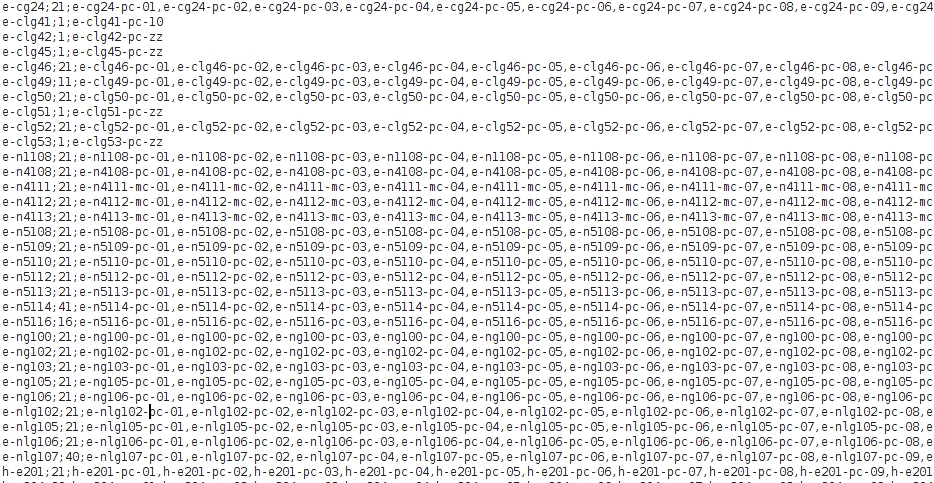
\includegraphics[scale=0.45]{reponseNagiosGetHostGroups.jpg}
	\caption{R\'eponse lors d'une requ\^ete de r\'ecup\'eration de salle}
	\label{annexe:reponseNagiosGetHostGroups}

\end{figure}

\subsubsection{Retour lors d'une r\'ecup\'eration des machines}

La r\'eponse~\ref{annexe:reponseNagiosGetResources} correspond \`a l'ex\'ecution de la requ\^ete~\ref{annexe:nagiosGetResources} sur le serveur contenant Nagios.

\begin{figure}[!ht]
	\centering
	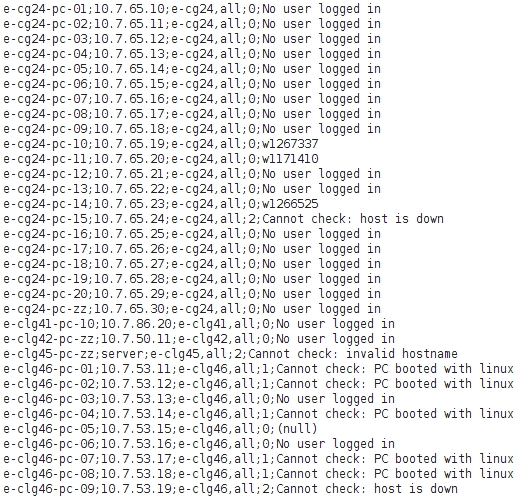
\includegraphics[scale=0.5]{reponseNagiosGetResources.jpg}
	\caption{R\'eponse lors d'une requ\^ete de r\'ecup\'eration des machines}
	\label{annexe:reponseNagiosGetResources}

\end{figure}

\subsubsection{Retour lors d'une r\'ecup\'eration des utilisateurs}

La r\'eponse~\ref{annexe:reponseNagiosGetUsersLogged} correspond \`a l'ex\'ecution de la requ\^ete~\ref{annexe:nagiosGetUsersLogged} sur le serveur contenant Nagios.

\begin{figure}[!ht]
	\centering
	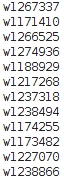
\includegraphics[scale=0.5]{reponseNagiosGetUsersLogged.jpg}
	\caption{R\'eponse lors d'une requ\^ete de r\'ecup\'eration des utilisateurs}
	\label{annexe:reponseNagiosGetUsersLogged}

\end{figure}

\chapter{Base de donn\'ees}
\label{chapterAnnexe:baseDeDonnees}

Cette annexe permet d'avoir une vue sur les relations entre tables ainsi que sur leur contenu.
Dans un premier temps, une description rapide des tables sera faite.
Ensuite, le diagramme de leur agencement les unes avec les autres sera donn\'e en entier.
Enfin, ce diagramme sera d\'ecoup\'e en diff\'erentes parties pour plus de visibilit\'e.

\subsubsection{Description des tables}

\noindent {\YuukouII} est compos\'e de 14 tables :

\begin{itemize}
	\item[\textbf{\textsf{yuukou\_rooms}}] contient les descriptions des salles informatiques;
	\item[\textbf{\textsf{yuukou\_resources}}] contient les descriptions des ordinateurs appartenant \`a une salle particuli\`ere;
	\item[\textbf{\textsf{yuukou\_users}}] contient les descriptions des utilisateurs;
	\item[\textbf{\textsf{yuukou\_last}}] contient les historiques de toutes les connexions pass\'ees sur les ordinateurs;
	\item[\textbf{\textsf{yuukou\_who}}] contient les historiques de toutes les connexions en cours sur les ordinateurs;
	\item[\textbf{\textsf{yuukou\_mapping\_location}}] contient les informations sur les diff\'erents campus de l'Universit\'e, le but \'etant de faire un lien avec la localisation de la table \textsf{yuukou\_rooms} et la description compl\`ete de cette localisation contenue dans la table de \textit{mapping};
	\item[\textbf{\textsf{yuukou\_mapping\_room}}] contient les diff\'erentes correspondances entre le nom des salles telles qu'elles sont appel\'ees dans {\YuukouII} et le nom des salles r\'ecup\'er\'ees avec les emplois du temps;
	\item[\textbf{\textsf{yuukou\_timetables}}] contient les diff\'erentes informations concernant un \'el\'ement de l'emploi du temps;
	\item[\textbf{\textsf{yuukou\_settings}}] contient les diff\'erentes informations de configuration de \YuukouII;
	\item[\textbf{\textsf{yuukou\_groups}}] contient les descriptions des groupes de logiciels;
	\item[\textbf{\textsf{yuukou\_software}}] contient les descriptions des logiciels;
	\item[\textbf{\textsf{yuukou\_groups\_software}}] contient les diff\'erents liens entre un groupe de logiciels et tous les logiciels les composant;
	\item[\textbf{\textsf{yuukou\_rooms\_groups}}] contient les diff\'erents liens entre les salles et tous les groupes de logiciels les composant;
	\item[\textbf{\textsf{yuukou\_roms\_software}}] contient les diff\'erents liens entre les salles et tous les logiciels, n'appartenant pas \`a un groupe de logiciels, les composant.
	
\end{itemize}


\subsubsection{Structure g\'en\'erale}

La figure~\ref{annexe:modeleGeneral} pr\'esente la structure g\'en\'erale du projet \YuukouII.
Elle s'articule en diff\'erentes sous-parties : la partie archivage, logicielle, emploi du temps, mapping et configuration.

\begin{figure}[!ht]
	\centering
	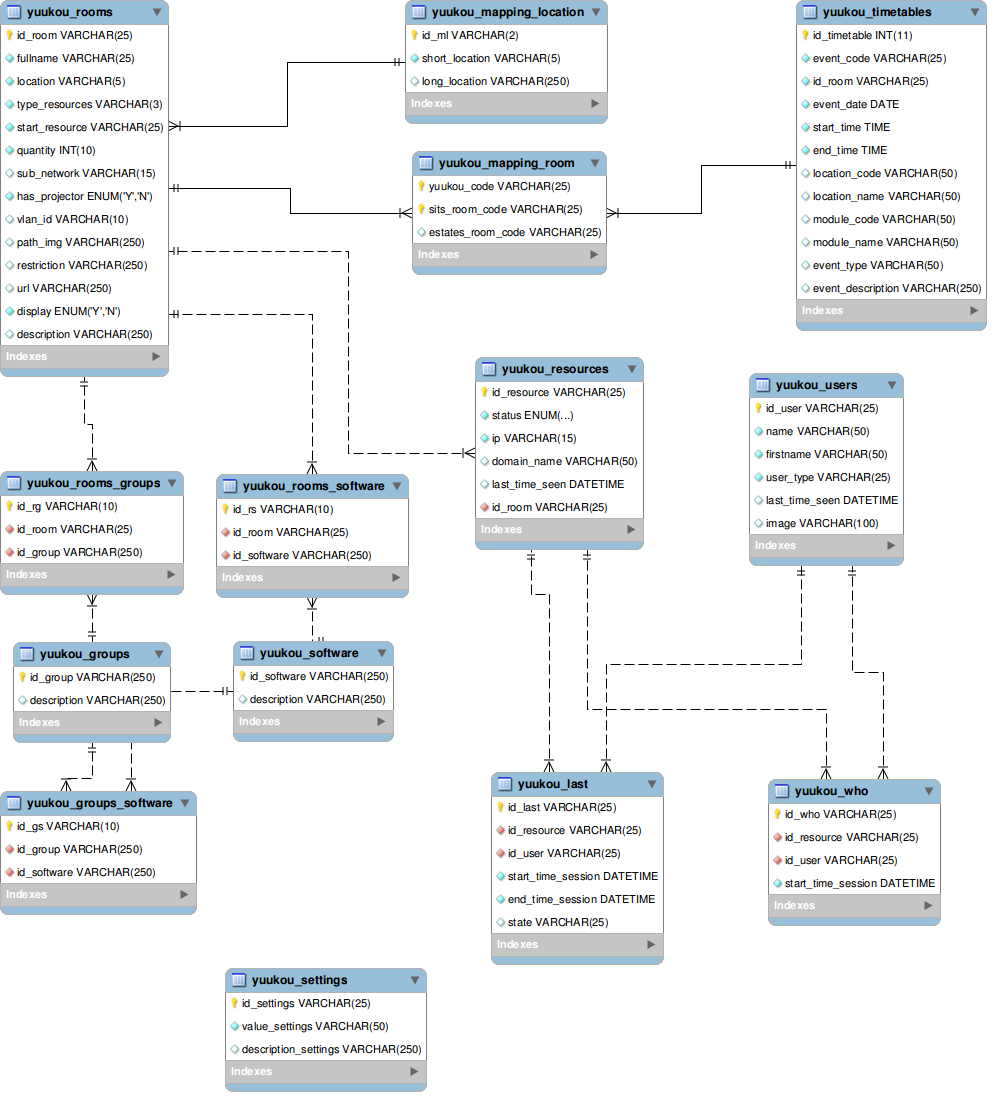
\includegraphics[scale=0.40]{modeleGeneral.png}
	\caption{Structure g\'en\'erale de la base de donn\'ees}
	\label{annexe:modeleGeneral}

\end{figure}

\clearpage

\subsubsection{Partie archivage}

La partie archivage a pour r\^ole le stockage des donn\'ees concernant d'une part l'historique des connexions actuelles et d'autre part, l'historique des connexions pass\'ees.

\begin{figure}[!ht]
	\centering
	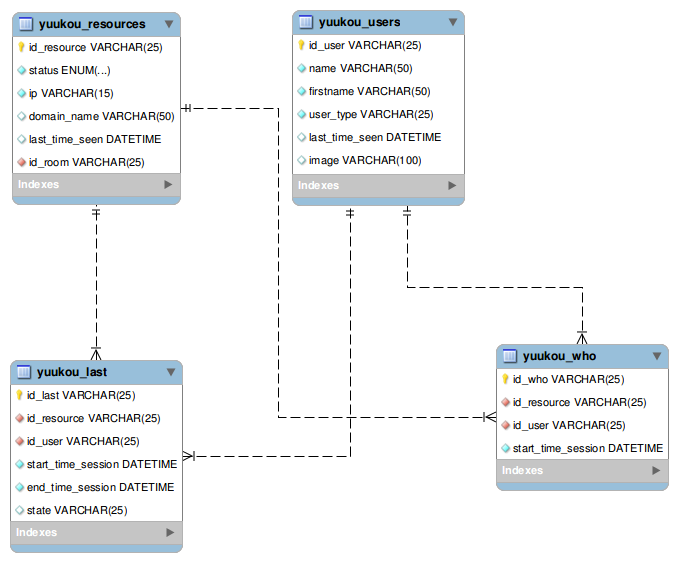
\includegraphics[scale=0.35]{modeleArchivage.png}
	\caption{Structure de la partie archivage de la base de donn\'ees}
	\label{annexe:modeleArchivage}

\end{figure}


\subsubsection{Partie logicielle}

La partie logicielle a pour r\^ole de lier les informations de configuration logicielle avec les salles informatiques de l'Universit\'e.

\clearpage

\begin{figure}[!ht]
	\centering
	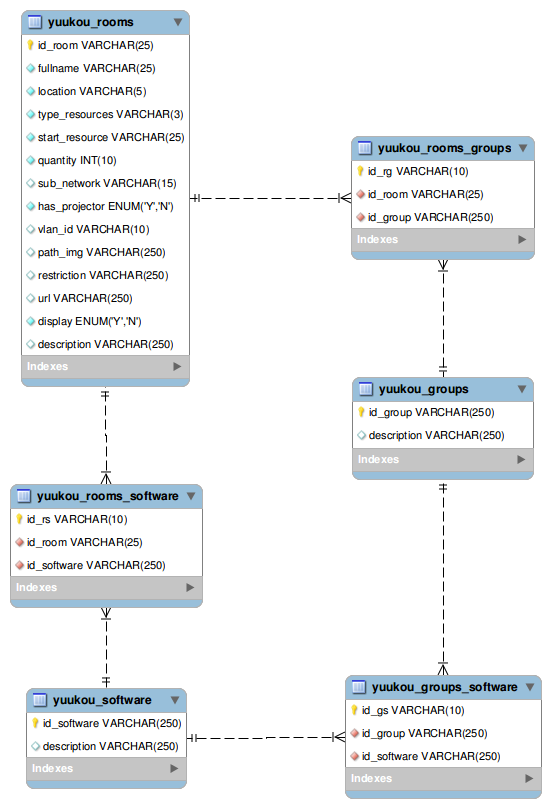
\includegraphics[scale=0.35]{modeleLogiciel.png}
	\caption{Structure de la partie logicielle de la base de donn\'ees}
	\label{annexe:modeleLogiciel}

\end{figure}


\subsubsection{Partie emploi du temps}

La partie emploi du temps a pour r\^ole de lier les informations d'emploi du temps \`a une salle en passant par une table de mapping faisant le lien entre le nom d'une salle dans {\YuukouII} et le nom d'une salle utilis\'e par les services centraux informatiques lors de la g\'en\'eration des emplois du temps.

\clearpage

\begin{figure}[!ht]
	\centering
	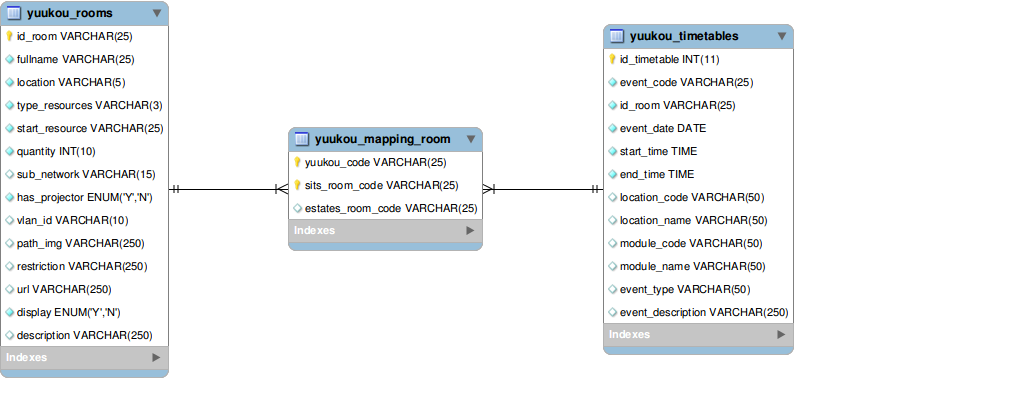
\includegraphics[scale=0.35]{modeleEmploiDuTemps.png}
	\caption{Structure de la partie emploi du temps de la base de donn\'ees}
	\label{annexe:modeleEmploiDuTemps}

\end{figure}

\subsubsection{Partie \textit{mapping} avec les salles}

La partie \textit{mapping} avec les salles a pour r\^ole de faire le lien entre la localisation d'une salle et les informations concernant cette localisation.

\begin{figure}[!ht]
	\centering
	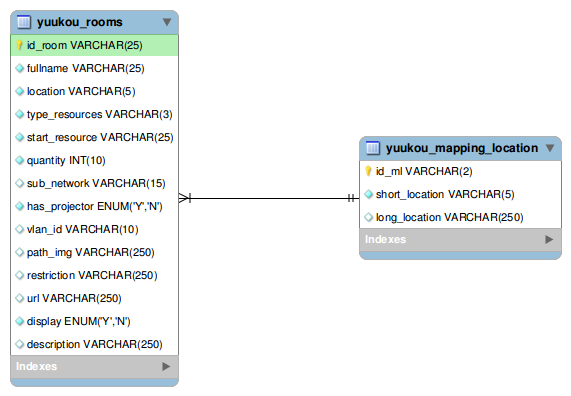
\includegraphics[scale=0.35]{modeleMapping.png}
	\caption{Structure de la partie \textit{mapping} de la base de donn\'ees}
	\label{annexemodeleMapping}

\end{figure}

\subsubsection{Partie configuration}

La partie configuration a pour r\^ole de stocker tous les param\`etres permettant de g\'erer un cycle du service Web pendant son ex\'ecution.

\begin{figure}[!ht]
	\centering
	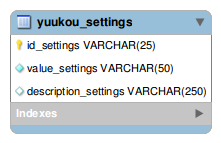
\includegraphics[scale=0.35]{modeleConfiguration.png}
	\caption{Structure de la partie configuration de la base de donn\'ees}
	\label{annexe:modeleConfiguration}

\end{figure}

\chapter{Exemples de retours JSON}
\label{chapterAnnexe:exempleJSON}

Cette annexe permet d'avoir une vue sur des exemples de retours corrects lors d'appels de fonctions du service Web.
Deux retours de m\'ethodes sont propos\'es ici.

Le code JSON~\ref{annexe:getsitesinformation} correspond au retour de l'appel \`a la fonction \textbf{getSitesInformation ()} du service Web.

\begin{figure}[!ht]
	\centering
	\lstinputlisting[language=JSON]{codes/getSitesInformation.json}
	\caption{Exemple de retour de la fonction \textbf{getSitesInformation ()}}
	\label{annexe:getsitesinformation}

\end{figure}

\clearpage

Le code JSON~\ref{annexe:getlistrooms} correspond au retour de l'appel \`a la fonction \textbf{getListRooms ()} du service Web.

\begin{figure}[!ht]
	\centering
	\lstinputlisting[language=JSON]{codes/getListRooms.json}
	\caption{Exemple de retour de  la fonction \textbf{getListRooms ()}}
	\label{annexe:getlistrooms}

\end{figure}

\end{appendices}

\clearpage


\addcontentsline{toc}{chapter}{Table des figures}
\listoffigures

\clearpage

\addcontentsline{toc}{chapter}{Liste des tableaux}
\listoftables

%~
\vfill

\noindent{\LARGE\textbf{R\'esum\'e}}

{\YuukouII} est un projet ayant pour objectif d'afficher la disponibilit\'e des salles informatiques de l'Universit\'e de Westminster \`a Londres.
Il consiste en la cr\'eation d'un service Web permettant de surveiller les ordinateurs de l'Universit\'e \`a l'aide de Nagios et d'archiver toutes les donn\'ees utiles permettant de donner la disponibilit\'e des salles.
Le projet offre diverses fonctionnalit\'es comme une connexion s\'ecuris\'ee, une r\'ecup\'eration des emplois du temps, de la configuration logicielle des salles, des informations concernant les utilisateurs \textit{via} LDAP ou encore la g\'en\'eration de graphes d'utilisation.

Le pr\'esent document rapporte le travail qui a \'et\'e effectu\'e dans le cadre du projet {\YuukouII} au sein de l'Universit\'e, projet r\'ealis\'e pour le stage de fin de cursus de Master 2 \`a l'Universit\'e de Franche-Comt\'e de Besan\c{c}on.

\vspace{0.5cm}

\noindent{\LARGE\textbf{Mots cl\'es}}

Java, service Web, JAX-WS, Nagios, surveillance, LDAP, Yuukou, GlassFish, NetBeans, MySQL.

\vspace{1cm}

\noindent{\LARGE\textbf{Abstract}}

{\YuukouII} is a project which enables to show the availability of computing laboratories within the University of Westminster in London.
During the project, a Web service was implemented to monitor computers of the University with Nagios and which can archive all useful data for showing rooms' availability.
The project provides various functionalities including secured connection, getting timetables of the University, software configuration of laboratories, information concerning users with LDAP or generation of graphical representation of laboratories utilization.

This document gives a view of the whole work done through the project {\YuukouII} within the University during the work placement of the second year of Master degree in the \textit{Universit\'e de Franche-Comt\'e} of Besan\c{c}on.

\vspace{0.5cm}

\noindent{\LARGE\textbf{Keywords}}

Java, Web service, JAX-WS, Nagios, monitoring, LDAP, Yuukou, GlassFish, NetBeans, MySQL.

\vfill


\end{document}
